%%%%%%%%%%%%%%%%%%%%%%%%%%%%%%%%%%%%%%%%%%%%%%%%%%%%%%%%%%%%%%%%%%%%%%%%%%%%%%%%
%2345678901234567890123456789012345678901234567890123456789012345678901234567890
%        1         2         3         4         5         6         7         8

\documentclass[twocolumn,10pt]{asme2ej}  % Comment this line out if you need a4paper

%\documentclass[a4paper, 10pt, conference]{ieeeconf}      % Use this line for a4 paper

%\IEEEoverridecommandlockouts                              % This command is only needed if 
% you want to use the \thanks command

%\overrideIEEEmargins                                      % Needed to meet printer requirements.

% See the \addtolength command later in the file to balance the column lengths
% on the last page of the document

% The following packages can be found on http:\\www.ctan.org
%\usepackage{graphicx}
\usepackage{graphics} % for pdf, bitmapped graphics files
\usepackage{epsfig} % for postscript graphics files
\usepackage{subcaption}
\usepackage[noadjust]{cite}
%\usepackage{mathptmx} % assumes new font selection scheme installed
%\usepackage{times} % assumes new font selection scheme installed
\usepackage{amsmath,amssymb,amsfonts,mathrsfs} % assumes amsmath package installed
\usepackage{algorithm,algpseudocode}
%\usepackage{booktabs}
\usepackage{balance}
\usepackage{tcolorbox}

% format for theorems etc.
\newtheorem{thm}{\bfseries Theorem}
\newtheorem{lem}{\bfseries Lemma}
\newtheorem{cor}{\bfseries Corollary}
\newtheorem{prop}{\bfseries Proposition}
\newtheorem{rem}{\bfseries Remark}

% format for argmin, argmax
\newcommand{\argmax}{\operatornamewithlimits{argmax}}

% format for cross-reference
\usepackage[capitalize]{cleveref}
\crefname{equation}{eq.}{eq.}
\Crefname{equation}{Eq.}{Eq.}
\crefname{thm}{theorem}{theorems}
\Crefname{thm}{Theorem}{Theorems}
\crefname{lem}{lemma}{lemmas}
\Crefname{lem}{Lemma}{Lemmas}
\crefname{cor}{corollary}{corollaries}
\Crefname{cor}{Corollary}{Corollaries}
\crefname{prop}{proposition}{propositions}
\Crefname{prop}{Proposition}{Propositions}
\crefname{rem}{remark}{remarks}
\Crefname{rem}{Remark}{Remarks}

% =====Macros for this manuscript===== %
\newcommand{\proto}{FIFO}
\newcommand{\lb}{\left\lbrace}
\newcommand{\rb}{\right\rbrace}
\newcommand{\X}{X}
\newcommand{\Z}{\mathcal{Z}}
\newcommand{\zb}{\mathbf{z}}
\newcommand{\B}{\mathcal{B}}
\newcommand{\Q}{\mathcal{Q}}
\newcommand{\K}{\mathcal{K}}
\newcommand{\xg}{x^g}
\newcommand{\fc}{frequently jointly strongly connected}
\newcommand{\thi}{^\text{th}}
\newcommand{\dnbhd}{direct neighbors}
\newcommand{\anbhd}{accessible neighbors}
\newcommand{\CB}{\textbf{\textit{CB}}}
\newcommand{\TL}{\textbf{\textit{TL}}}

%=====todonotes===== %
\usepackage{todonotes}
\usepackage{soul}
\definecolor{smoothgreen}{rgb}{0.7,1,0.7}
\sethlcolor{smoothgreen}

\newcommand{\todopara}[1]{\vspace{0px} %
	\todo[inline, color=black!10]{\textbf{[Paragraph:]} {#1}} %
}
\newcommand{\todonote}[1]{\vspace{0px} %
	\todo[inline, color=green!30]{\textbf{[Note:]} {#1}} %
}
\newcommand{\todoQ}[1]{\vspace{0px} %
	\todo[inline, color=orange!50]{\textbf{[Note:]} {#1}} %
}
\newcommand{\todohere}[1]{\hl{(\textbf{TODO:} #1)}}

\newcommand{\hidetodos}{
	\renewcommand{\todopara}[1]{}
	\renewcommand{\todonote}[1]{}
	\renewcommand{\todoQ}[1]{}
	\renewcommand{\todohere}[1]{}
}

\title{\LARGE \bf
	Distributed Bayesian Filter using Measurement Dissemination for Multiple UGVs with Dynamically Changing Interaction Topologies}
% Measurement Dissemination-based Distributed Bayesian Filter Under Dynamically Changing Interaction Topologies for Target Tracking
%Estimation of Moving Targets Using Distributed Bayesian Filter Under Dynamically Changing Networks
	%Distributed Bayesian Filter Under Dynamically Changing Interaction Topologies}


%%% first author
\author{Chang Liu
	\affiliation{		
		Department of Mechanical Engineering\\
		University of California, Berkeley\\
		Berkeley, CA 94720\\
		Email: changliu@berkeley.edu
	}	
}
%\thanks{The first two authors have equally contributed to this research.}

%%% second author
%%% remove the following entry for single author papers
%%% add more entries for additional authors
\author{Shengbo Eben Li\thanks{Address all correspondence to this author.}
	\affiliation{Department of Automotive Engineering\\ 
		Tsinghua University\\
		Beijing, China 100084\\
		Email: lisb04@gmail.com
	}
}

%%% third author
%%% remove the following entry for single author papers
%%% add more entries for additional authors
\author{J. Karl Hedrick
	\affiliation{
		Department of Mechanical Engineering\\
		University of California, Berkeley\\
		Berkeley, CA 94720\\
		Email: khedrick@me.berkeley.edu
	}
}


\begin{document}
	
	%\hidetodos % hide all todos 
	
	\maketitle
	\thispagestyle{empty}
	\pagestyle{empty}
	
	%\setlength{\belowcaptionskip}{-10pt} % set the spacing between figure and text
	
	%%%%%%%%%%%%%%%%%%%%%%%%%%%%%%%%%%%%%%%%%%%%%%%%%%%%%%%%%%%%%%%%%%%%%%%%%%%%%%%%
	\todohere{modify abstract, intro, and sec 2 based on the meeting with SL.}
	\begin{abstract}
		This paper presents a novel distributed Bayesian filtering algorithm using measurement dissemination for multiple unmanned ground vehicles (UGVs) with dynamically changing interaction topologies.
		Different from statistics dissemination-based approaches that transmit posterior distributions or likelihood functions, this algorithm relies on the measurement dissemination scheme, which significantly reduces the transmission burden between each pair of UGVs. 
%		, called Full-In-and-Full-Out (\proto) protocol. 		
%		\todohere{explain how to disseminate}
%		that transmit posterior distributions or likelihood functions, each UGV under {\proto} only sends a communication buffer and a track list to neighboring agents,	
%		The information exchange among UGVs relies on a measurement dissemination scheme, called Full-In-and-Full-Out (\proto) protocol. 		
		Each UGV only sends a communication buffer and a track list to neighboring agents.
		A communication buffer contains its own measurements and the received ones from other UGVs.
		And a track list is used to trim all measurements in the buffer to reduce communication overhead.
		%		latest available measurements to neighboring nodes, 
%		 to scale linearly with the size of the network.
		Under the condition that the interaction topologies are \fc,
%		 union of undirected switching topologies is connected frequently enough,
		each UGV's measurements can be disseminated over the network within finite time.
%		The \proto-based DBF algorithm is then developed to estimate individual probability density function (PDF) with the application for target tracking.
%		in a static environment. 
		The proposed DBF algorithm is proved to achieve consistent state estimation.
%		, of this algorithm is proved that each individual estimate of target position converges in probability to the true target position.
		The effectiveness of this algorithm is validated by comparing with consensus-based distributed filters and the centralized filter in multi-target tracking simulations.
%		Simulation results on multiple target tracking demonstrate that the proposed DBF achieves comparable tracking performance as a centralized filter and has more superior uncertainty reduction performance than the commonly used consensus-based filter.
	\end{abstract}
	
	\section{INTRODUCTION}
	
%	Unmanned ground vehicles (UGV) that operate without on-board operators have been used for many applications that are inconvenient, dangerous, or impossible to human. 
	Estimation using a group of networked UGVs has been utilized to collectively measure environment status \cite{hedrick2011tools}, such as intruder detection \cite{chamberland2007wireless}, and signal source seeking \cite{atanasov2015distributed}, and pollution field estimation \cite{madhag2017distributed}. 
	Filtering methods such as the Kalman Filter, extended Kalman filter, and the particle filter have been widely adopted \cite{thrun2005probabilistic}.
%	Several techniques have been developed for distributed estimation, including distributed linear Kalman filter (DKF) \cite{2005distributed}, distributed extended Kalman filter \cite{madhavan2004distributed}, and distributed particle filter \cite{gu2007distributed}. 
	The most generic filtering scheme is the Bayesian filter, which can be applied for nonlinear systems with arbitrary noise distributions \cite{bandyopadhyay2014distributed,julian2012distributed}.
	In fact, under the assumption of linearity and Gaussian noise, a Bayesian filter can be reduced to the Kalman filter \cite{chen2003bayesian}.
	For general nonlinear systems, the particle filter is usually utilized as the numerical implementation of the Bayesian filter \cite{chen2003bayesian}, due to the advantage in computation.
	This paper focuses on the networked Bayesian filter for target tracking under dynamically changing interaction topologies.
	
	The interaction topology plays a central role on the design of the networked Bayesian filter, of which two types are widely investigated in literature: the centralized filter and the distributed filter.
	In the former, local statistics estimated by each agent is transmitted to a single fusion center, where a global posterior distribution is calculated at each filtering cycle \cite{zuo2006bandwidth,vemula2006target}. 
	In the latter, each agent individually executes distributed estimation and the agreement of local estimates is achieved by certain consensus strategies \cite{jadbabaie2003coordination,ren2005consensus,olfati2007consensus}.
	In general, the distributed filters are more suitable in practice since they do not require a fusion center with powerful computation capability and are more robust to changes in network topology and link failures. 
	So far, the distributed filters have two mainstream schemes in terms of the transmitted data among agents, i.e., the \textit{statistics dissemination} (SD) and the \textit{measurement dissemination} (MD). 
	In the SD scheme, each agent exchanges statistics such as posterior distributions and likelihood functions within neighboring nodes \cite{hlinka2013distributed}. 
	In the MD scheme, instead of exchanging statistics, each agent sends measurements to neighboring nodes. 
	
%	The pioneering work of statistics dissemination scheme can date back to the 80s of last century \todohere{reference}. 
%	Later, \todohere{reference} have considerably advanced the study of this scheme in the field of distributed estimation. 
	Statistics dissemination scheme has gained increasing interest and been widely investigated during last decade.
	Madhavan et al. (2004) presented a distributed extended Kalman filter for nonlinear systems \cite{madhavan2004distributed}. This filter was used to generate local terrain maps by using pose estimates to combine elevation gradient and vision-based depth with environmental features. Olfati-Saber (2005) proposed a distributed linear Kalman filter (DKF) for estimating states of linear systems with Gaussian process and measurement noise \cite{2005distributed}. Each DKF used additional low-pass and band-pass consensus filters to compute the average of weighted measurements and inverse-covariance matrices. 
%	Sheng et al. (2005) proposed a multiple leader-based distributed particle filter with Gaussian Mixer for target tracking \cite{sheng2005distributed}. Sensors are grouped into multiple uncorrelated cliques, in each of which a leader is assigned to perform particle filtering and the particle information is then exchanged among leaders. 
	Gu (2007) proposed a distributed particle filter for Markovian target tracking over an undirected sensor network \cite{gu2007distributed}. Gaussian mixture models (GMM) were adopted to approximate the posterior distribution from weighted particles and the parameters of GMM were exchanged via average consensus filter. 
	Hlinka et al. (2012) proposed a distributed method for computing an approximation of the joint (all-sensors) likelihood function by means of weighted-linear-average consensus algorithm when local likelihood functions belong to the exponential family of distributions \cite{hlinka2012likelihood}. Saptarshi et al. (2014) presented a Bayesian consensus filter that uses logarithmic opinion pool for fusing posterior distributions of the tracked target \cite{bandyopadhyay2014distributed}. Other examples can be found in \cite{julian2012distributed} and \cite{beaudeau2012target}. 
%	Generally, this scheme can be further categorized into two types: leader-based and consensus-based. In the former, statistics is sequentially passed and updated along a path formed by active UGVs, called leaders. Only leaders perform filtering based on its own measurement and received measurements from local neighbors \cite{sheng2005distributed}. In the latter, every UGV diffuses statistics among neighbors, via which global agreement of the statistics is achieved by using consensus protocols \cite{olfati2007consensus,ren2005consensus,jadbabaie2003coordination}. 
	
	
	Despite the popularity of statistics dissemination, exchanging statistics can consume high communication resources. 
	One remedy is to approximate statistics with parametric models, e.g., Gaussian Mixture Model \cite{sheng2005distributed}, which can reduce communication burden to a certain extent. 
	However, such manipulation increases the computation burden of each agent and sacrifices filtering  accuracy due to approximation.
	The measurement dissemination scheme is an alternative solution to address the issue of exchanging statistics. 
	An early work on measurement dissemination was done by Coates et al. (2004), who used adaptive encoding of observations to minimize communication overhead \cite{coates2004distributed}. Ribeiro et al. (2006) exchanged quantized observations along with error-variance limits considering more pragmatic signal models \cite{ribeiro2006bandwidth}.
	A recent work was conducted by Djuric et al. (2011), who proposed to broadcast raw measurements to other agents, and therefore each agent has a complete set of observations of other agents for executing particle filtering \cite{djuric2011non}.  
	A shortcoming of aforementioned works is that their communication topologies are assumed to be a fixed and complete graph that every pair of distinct agents is constantly connected by a unique edge. 
	In many real applications, the interaction topology may change dynamically due to unreliable links, external disturbances and/or range limits \cite{xiao2008asynchronous}.
%	The communication links between UGVs may be unreliable due to disturbances or communication range limitations. 
%	If the information is being exchanged by direct sensing, the locally visible neighbors of a vehicle will likely change over time. 
	In such cases, dynamically changing topologies can cause random packet loss, variable transmission delay, and out-of-sequence measurement issues (OOSM) \cite{xia2009networked}, thus decreasing the performance of distributed estimation.
%	, and even leading to inconsistency and non-consensus. 
	Leung et al. (2010) explored a decentralized Bayesian filter for dynamic robot networks \cite{leung2010decentralized}.
	The algorithm was shown to achieve centralized-equivalent filtering performance in simulations. 
	However, it required the communication of both measurements and statistics, which could incur large communication overhead.
		
	The main contribution of the paper is that we present a measurement dissemination-based distributed Bayesian filtering (DBF) method for a group of networked UGVs with dynamically changing interaction topologies. 
	In our previous work \cite{liu2016distributed}, we have proposed a Latest-In-and-Full-Out (LIFO) protocol for data exchange and developed a LIFO-based DBF. 
	However, it only applies to static target with simple binary sensor model.
	In this work, we introduce the concept of the track list and extend our methods to time-varying topologies and more general sensor models.
	The measurement dissemination scheme uses the so-called Full-In-and-Full-Out (\proto) protocol, under which each UGV is only allowed to broadcast observations to its neighbors by using single-hopping.
	An individual Bayesian filter is implemented locally by each UGV after exchanging observations using \proto.
	Under the condition that the topologies is \fc, {\proto} can disseminate measurements over the network within a finite time.
%	two properties are achieved: (1) {\proto} can disseminate observations over the network within finite time; (2) \proto-based DBF guarantees the consistency of estimation that each individual estimate of target position converges in probability to the true target position as the number of observations tends to infinity. 
	The main benefit of using {\proto} is on the reduction of communication burden while avoiding the OOSM issue and ensuring that no information loss occurs.
%	, with the transmission data volume scaling linearly with the size of the UGV network. 
	
	The rest of this paper is organized as follows: 
	\Cref{sec:prob} formulates the target tracking problem using multiple UGVs;
	\Cref{sec:\proto} proposes the {\proto} protocol for measurement communication in dynamically changing interaction topologies;
	\Cref{sec:\proto-dbf} introduces \proto-based DBF algorithm and track list;
%	 where the consistency of estimation is proved;
	simulation results are presented in \cref{sec:sim} and \cref{sec:conclu} concludes the paper.
	\section{Problem Formulation}\label{sec:prob}
\begin{figure}%[thpb]
	\centering
	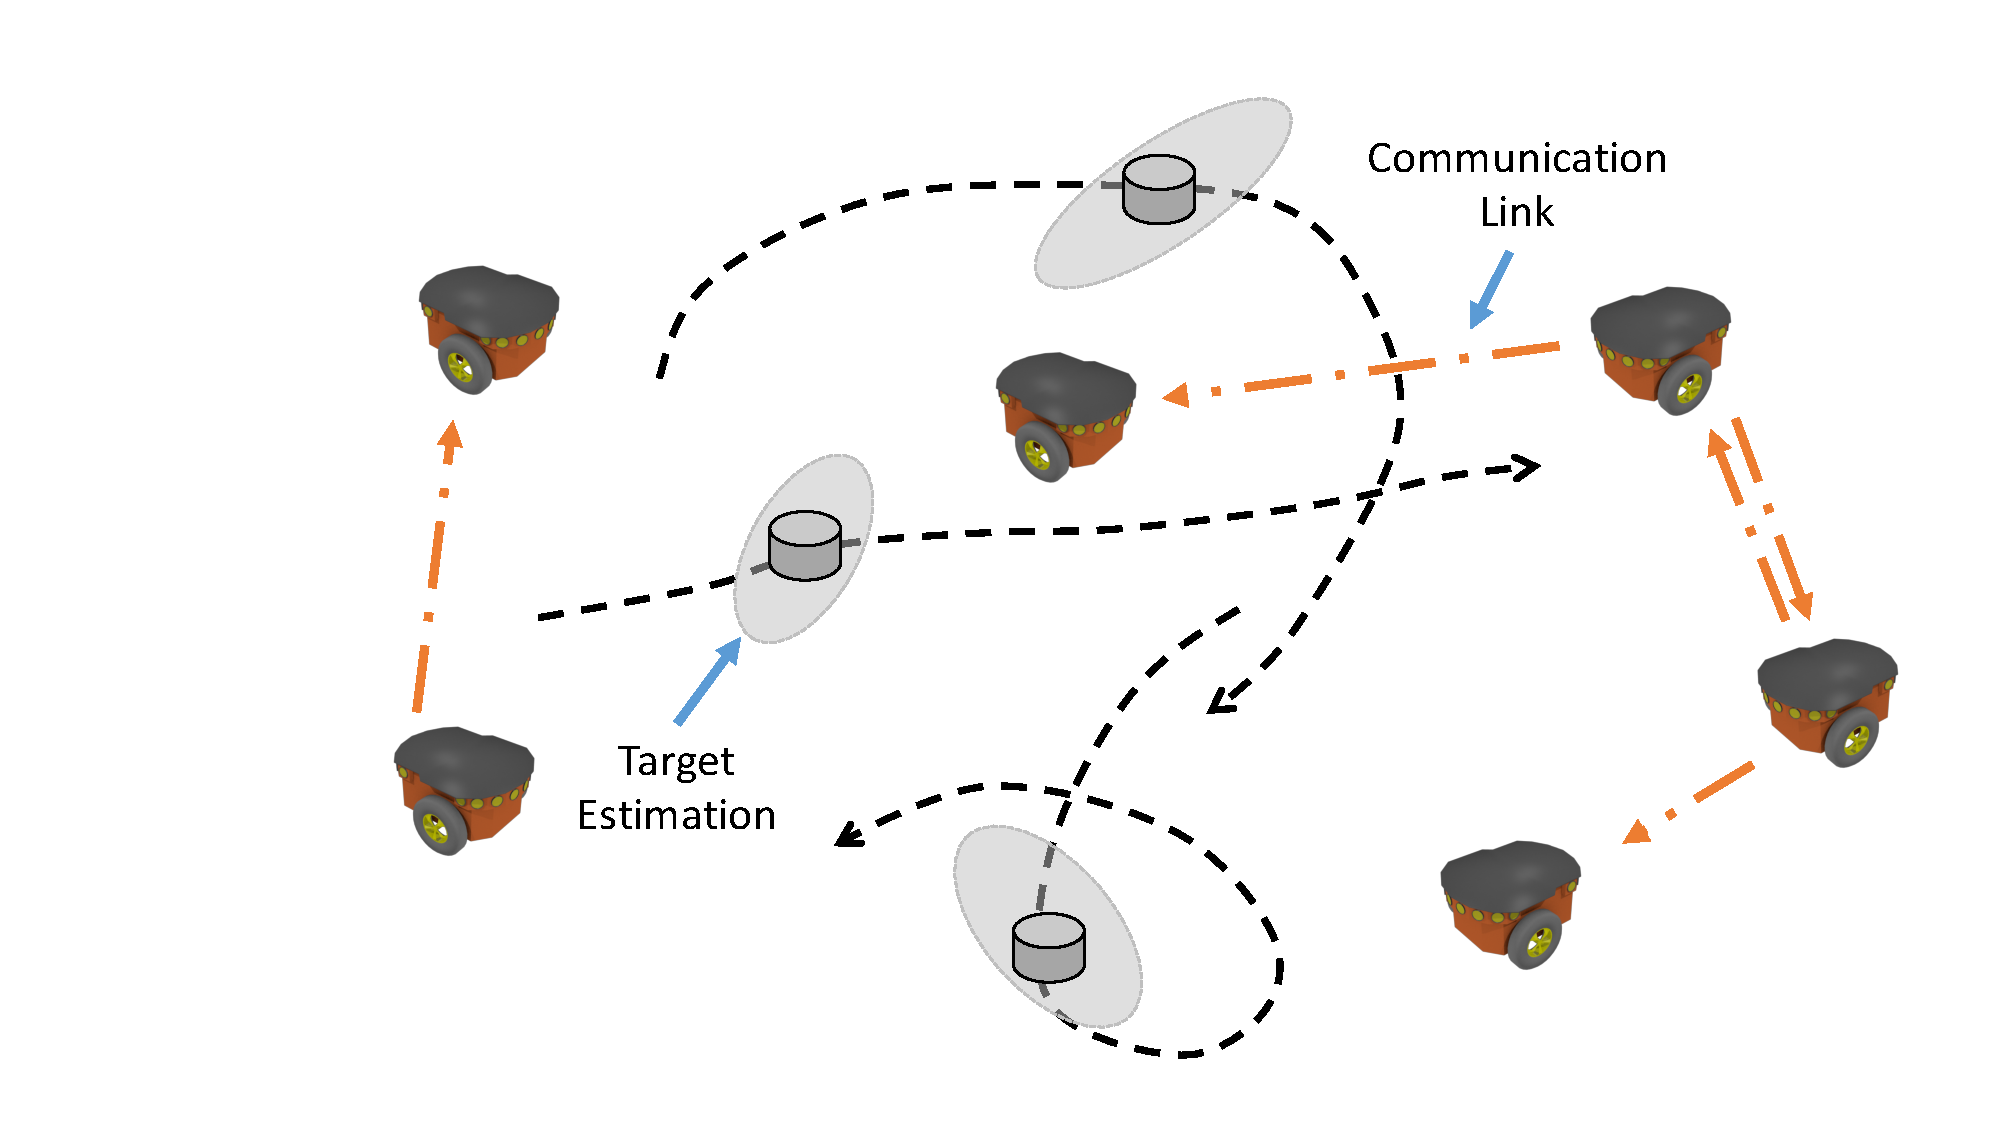
\includegraphics[width=0.45\textwidth]{figures/scenario}
	\caption{Target tracking scenario. The interaction topology is dynamically changing and UGVs can only communicate with neighboring UGVs.}
	\label{fig:scenario}
	%		\vspace{-1em}]
\end{figure}
%	\section{\proto Protocol for Dynamically Changing Interaction Topologies}\label{sec:lifo}
	Consider a network of $N$ UGVs in a bounded two-dimensional space $S$, as shown in \cref{fig:scenario}.
	The interaction topology can be dynamically changing due to limited communication range, team reconfiguration, or intermittently link failure.
	Each UGV is equipped with a sensor for target detection. 
	Due to the limit of communication range, each UGV can only exchange sensor measurements with its local neighbors. 
%	The Bayesian filter is run locally on each UGV based on its own measurements and the received measurements from other UGVs to estimate the target position in $S$.
	Every UGV locally runs a Bayesian filter to estimate the target position in $S$ utilizing its own measurements and the received measurements from other UGVs. 
%	Since this work is focused on the distributed Bayesian filter for target localization, we assume that UGVs' states are accurately known.
%	An illustration of the scenario is shown in \cref{fig:scenario}.
	
	\subsection{Target and Sensor Model}
	%Probabilistic Model of Binary Sensor}
	%In this paper, distributed Bayesian filter is used to estimate the true target position by a network of binary sensors.
	The target motion uses a stochastic discrete-time model: % that can be described by
	
	\begin{equation}
		\small
		\label{eqn:tar_motion_model}
		\xg_{k+1}=f(\xg_k,v_k), %,u^g_k
		%x_{k+1}=A_kx_k+B_ku^g_k+\epsilon,
	\end{equation}\normalsize
	where the superscript $g$ represents the target and $\xg_k\in S$ is the target position at time $k$;
	$v_k$ is the white process noise.
	% and $u^g_k$ is the target control input.
	%$A_k\in\mathbb{R}^{2\times 2},\;B_k\in\mathbb{R}^{2\times 2}$ and $\epsilon$ denotes the process noise.
	
	%Each UGV constantly measures the target position and the 
	The sensor measurement is described by a stochastic model:
	\small\begin{equation}\label{eqn:meas_model}
		z^i_k = h_i(\xg_k,x^i_k)+w^i_k,
	\end{equation}\normalsize
	where the superscript $i\in\left\lbrace 1,\dots,N\right\rbrace$ represents the index of the UGV; $x^i_k\in S$ is the sensor position and $w^i_k$ is the white measurement noise.
	% $x^i_k=[x^i_k;\theta^i_k]$ represents the sensor state, consisting of the sensor position $x^i_k$ and direction $\theta^i_k$.
	The measurement function $h_i$ depends on the type of the sensor. 
	%Let $\mathcal{F}(x^i_k)$ denote the sensor's sensing domain, 
	
%	The conditional probability, denoted by $P(z^i_k|x^g_k;x^i_k)$, of obtaining a certain measurement $z^i_k$ conditioning on the target and sensor states is critical to designing the Bayesian filter \cite{thrun2005probabilistic}. 
	The design of the Bayesian filter relies on the conditional probability of obtaining a certain measurement $z^i_k$ given the current target and sensor states, which is denoted by $P(z^i_k|x^g_k;x^i_k)$ \cite{thrun2005probabilistic}. 	
%	We define $P(z^i_k|x^g_k;x^i_k)$ as this conditional probability.
%	 of $z^i_k$ given the sensor state $x^i_k$ and the target state $\xg_k$. 
	The conditional probability $P(z^i_k|x^g_k;x^i_k)$ depends on both $h_i$ and $w^i_k$ in \Cref{eqn:meas_model}.
	For example, if $w^i_k$ is a zero-mean Gaussian white noise with covariance $\Gamma_k^i$, then $P(z^i_k|x^g_k;x^i_k)$ can be described as $P(z^i_k|x^g_k;x^i_k)=N(h_i(\xg_k,x^i_k),\Gamma_k^i)$.
%	\small\begin{equation*}%\label{eqn:prob_sensor3}
%		P(z^i_k|x^g_k;x^i_k)=\mathcal{N}(h_i(\xg_k,x^i_k),\Gamma_k^i).
%	\end{equation*}\normalsize
	For non-Gaussian noise, such as Poisson noise or Cauchy noise \cite{kitagawa1996monte}, $P(z^i_k|x^g_k;x^i_k)$ can also be similarly defined (for the purpose of simplicity, $P(z^i_k|x^g_k;x^i_k)$ is shorted as $P(z^i_k|x^g_k)$ for the rest of the paper). 
	It should be noted that this work is not confined to any specific distribution of the noise.
	The measurement function $h_i$ for several typical sensors are listed as follows \cite{bishop2010optimality}:
	
	\textbf{Range-only sensors:} 
	%when the target is within the sensor's sensing domain, 
	$h_i$ is a function of the relative Euclidean distance between the sensor and the target:
	%\begin{subequations}
	%	\begin{align}
	\small\begin{equation*}%\label{eqn:ran_only}
		h_i(\xg_k,x^i_k)=\|\xg_k-x^i_k\|_2,
	\end{equation*}	\normalsize
	%\begin{equation}\label{eqn:ran_only}
	%h_i(\xg_k,w^i_k;x^i_k)=
	%\begin{cases}
	%\|\xg_k-x^i_k\|_2+w^i_k\; &\text{if}\, \xg_k\in\mathcal{F}(x^i_k)\\
	%\emptyset\; &\text{if}\, \xg_k\notin\mathcal{F}(x^i_k)
	%\end{cases},
	%\end{equation}		
	where $\|\cdot\|_2$ is the Euclidean distance in $S$.
	%		w^i_k&\sim\mathcal{N}(0,\sigma^i),
	%	\end{align}
	%\end{subequations}
	
	\textbf{Bearing-only sensors:} 
	%when the target is within the sensor's sensing domain, 
	$h_i$ is a function of the relative bearing between the sensor and the target:
	\small\begin{equation*}
		h_i(\xg_k,x^i_k)=\measuredangle (\xg_k-x^i_k),
	\end{equation*}\normalsize
	%\begin{equation}
	%h_i(\xg_k,w^i_k;x^i_k)=
	%\begin{cases}
	%\measuredangle (\xg_k-x^i_k)+w^i_k\; &\text{if}\, \xg_k\in\mathcal{F}(x^i_k)\\
	%\emptyset\; &\text{if}\, \xg_k\notin\mathcal{F}(x^i_k)
	%\end{cases},
	%\end{equation}
	where $\measuredangle$ denotes the angle from the sensor to the target.
	
	\textbf{Range-bearing sensors:} $h_i$ includes both the relative distance and bearing: % between the sensor and the target:
	\small\begin{equation*}
		h_i(x^g_k,x^i_k)=x^g_k-x^i_k.
	\end{equation*}\normalsize
	
%	\subsection{Target and Sensor Model}
%	The target motion takes a deterministic discrete-time model:	
%	\begin{equation}
%		\small
%		\label{eqn:tar_motion_model}
%		x^g_{k+1}=f(x^g_k),
%	\end{equation}\normalsize
%	where $x^g_k\in \mathbb{R}^{2}$ denotes the target position at time $k$; $u^g_k$ represents the control input of the target.
%	
%	Each UGV constantly measures the target position and the sensor measurement of $i\thi$ UGV can be described by a stochastic model:
%	\begin{equation}
%		z^i_k = g_i(x^g_k,w^i_k;y^i_k),
%	\end{equation}
%	where $w^i_k$ is the white measurement noise and $y^i_k=[x^i_k;\theta^i_k]$ represents the sensor state, consisting of the sensor position $x^i_k$ and direction $\theta^i_k$.
%	$g_i$ depends on the type of the sensor. Let $\mathcal{F}(y^i_k)$ denote the sensor field of view (FOV), $g_i$ for several typical sensor types can be defined as follows:
%	
%	\textbf{Range-only sensors:} when the target is within the sensor's FOV, the measurement only depends on the relative distance between the sensor and the target.
%	\begin{equation*}%\label{eqn:ran_only}
%		h_i(\xg_k,x^i_k)=\|\xg_k-x^i_k\|_2,
%	\end{equation*}	
%%	\begin{equation}
%%		g_i(x^g_k,w^i_k;x^i_k)=
%%		\begin{cases}
%%			\|x^g_k-x^i_k\|_2+w^i_k\; &\text{if}\, x^g_k\in\mathcal{F}(y^i_k),\\
%%			\emptyset\; &\text{if}\, x^g_k\notin\mathcal{F}(y^i_k).
%%		\end{cases}
%%	\end{equation}
%	
%	\textbf{Bearing-only sensors:} when the target is within the sensor's FOV, the measurement only depends on the relative bearing between the sensor and the target.
%	\begin{equation}
%		g_i(x^g_k,w^i_k;x^i_k)=
%		\begin{cases}
%			\measuredangle (x^g_k-x^i_k)+w^i_k\; &\text{if}\, x^g_k\in\mathcal{F}(y^i_k),\\
%			\emptyset\; &\text{if}\, x^g_k\notin\mathcal{F}(y^i_k).
%		\end{cases}
%	\end{equation}
%	
%	\textbf{Range-bearing sensors:} $h_i$ includes both the relative distance and bearing: % between the sensor and the target:
%	\begin{equation*}
%		h_i(x^g_k,x^i_k)=x^g_k-x^i_k.
%	\end{equation*}
%	
%%	\textbf{Range-bearing sensors:} when the target is within the sensor's FOV, the measurement is the relative distance and bearing between the sensor and the target.
%%	\begin{equation}
%%		g_i(x^g_k,w^i_k;x^i_k)=
%%		\begin{cases}
%%			x^g_k-x^i_k+w^i_k\; &\text{if}\, x^g_k\in\mathcal{F}(y^i_k),\\
%%			\emptyset\; &\text{if}\, x^g_k\notin\mathcal{F}(y^i_k).
%%		\end{cases}
%%	\end{equation}
%		
%	A probabilistic sensor model that describes the conditional probability of a certain measurement given sensor and target state is a key component for Bayesian filtering.
%	We define a likelihood function to represent the probability of the target being detected by a sensor:
%	\small\begin{equation}\label{eqn:prob_sensor1}
%		p^i_{1,k}=P(z^i_k\neq\emptyset|x^g_k;x^i_k)\in \left[0,1\right],\; x^g_k\in S,
%	\end{equation}\normalsize
%	where $x^i_k$ is the $i\thi$ sensor's position.
%	%; $X^g$ represents the set of all possible target positions.
%	Correspondingly, the likelihood function for no target being detected is:
%	\small\begin{equation}\label{eqn:prob_sensor0}
%		p^i_{0,k}=P(z^i_k=\emptyset|x^g_k;x^{i}_k)=1-p^i_{1,k}.
%	\end{equation}\normalsize
%	%\Cref{eqn:bin_sensor} actually defines a binary sensor model parameterized by $x^g_k$ and $x^R_k$.
%	
%	The combination of \Cref{eqn:prob_sensor1} and \Cref{eqn:prob_sensor0} forms the probabilistic model for a sensor.
%	If $w^i_k$ is a zero-mean Gaussian white noise, then the probabilistic sensor model can be described as
%	\begin{equation}		
%		\begin{cases}
%			p^i_{1,k}\sim\mathcal{N}(\bar{z}^i_k,\Sigma^i_k) & \text{if}\,x^g_k\in\mathcal{F}(y^i_k)\\
%			p^i_{1,k}=0 & \text{if}\,x^g_k\in\mathcal{F}(y^i_k),
%		\end{cases}
%	\end{equation}
%	where $\bar{z}^i_k$ is the nominal value of the measurement and equals $\|x^g_k-x^i_k\|$ and $\measuredangle(x^g_k-x^i_k)$ for range-only and bearing-only sensors, correspondingly.
%	
%	Consequently,
%	\begin{equation}
%		p^i_{0,k}=
%		\begin{cases}
%			0 & \text{if}\,x^g_k\in\mathcal{F}(y^i_k)\\
%			1 & \text{if}\,x^g_k\in\mathcal{F}(y^i_k).
%		\end{cases}
%	\end{equation}
	
%	For the purpose of simplicity, we will not explicitly write $x^{i}_k$ in the sensor model (\Cref{eqn:prob_sensor1,eqn:prob_sensor0}) for the rest of the paper.
	
%	\begin{rem}
%		Given the knowledge of current target and UGV positions, the current measurement by each UGV can be considered conditionally independent from its own past measurements and those by other UGVs \cite{bourgault2003optimal}.
%	\end{rem}
	
%	\begin{rem} 
%		The proposed {\proto} protocol and the consistency property to be described in \cref{sec:\proto-dbf} are applicable for general sensors, not limited to the ones described in this section. In addition, they do not rely on the Gaussian noise assumption.
%	\end{rem}
	
	\subsection{Graphical Model of Interaction Topology}
	%The UGV network is always assumed to be connected, i.e., there exists a path, either direct or indirect, between every pair of UGVs.
	%Under this assumption, consider an undirected and fixed graph 
	We consider a simple\footnote{A (directed/undirected) graph $G=(V,E)$ is \textit{simple} if it has no self-loops (i.e., $\left( i,j\right)\in E\,\text{only if } i\neq j$) or multiple edges with the same source and target nodes (i.e., $E$ only contains distinct elements).} graph $G=(V,E)$ to represent the interaction topology of N networked UGVs, where the vertex set $V=\left\lbrace 1,\dots,N\right\rbrace $ represents the index set of UGVs and $E=V\times V$ denotes the edge set. 
	For the purpose of narrative simplicity, we use directed graphs to describe our approach in this work.
%	The approach can conveniently apply to undirected graphs, which can be treated as bidirectional directed graphs.
	The undirected graphs can actually be treated as bidirectional directed graphs.
	
	The \textit{adjacency matrix} $A=\left[ a_{ij}\right] $ of the graph $G$ describes the interaction topology:
	\small\begin{equation*}
		a_{ij}=\begin{cases}
			1& \text{if}\;\left(i,j\right)\in E\\
			0& \text{if}\;\left(i,j\right)\notin E
		\end{cases},
	\end{equation*} \normalsize
	where $a_{ij}$ is the entry on the $i\thi$ row and $j\thi$ column of the adjacency matrix. 
	The notation $a_{ij}=1$ indicates that the $i\thi$ UGV can directly communicate to the $j\thi$ UGV and $a_{ij}=0$ indicates no direct communication from $i$ to $j$.
%	 a communication link exists from the $i\thi$ to $j\thi$ UGV and $m_{ij}=0$ indicates no communication from $i$ to $j$.
	 A directed graph is \textit{strongly connected} if there is a directed path connecting any two arbitrary vertices in $V$. %\footnote{An undirected graph with this property is called a \textit{connected} graph.}.
%	\cref{fig:com_topo} illustrates three types of typical simple directed topologies: ring \cite{lawton2003decentralized}, line \cite{liu2010simple}, and star \cite{thatte2008sensor}. 
%	All of them are represented by simple and undirected graphs.
	
%	The interaction topology can be dynamically changing due to limited communication range, varying team formation or link failure.
%	Let $\bar{G}=\left\lbrace G_1,G_2,\dots,G_L\right\rbrace $ denote the set of all possible simple and undirected graphs defined for the network of UGVs.
%	Let $\bar{G}$ denote the set of all possible simple and undirected graphs defined for the network of UGVs.
%	Let $\bar{G}$ denote the set of all possible simple directed graphs\footnote{For undirected graphs, we consider the set of simple undirected graphs.} defined over the network of UGVs.
%	It is easy to know that $\bar{G}$ has finite elements.
%	The adjacency matrix associated with a graph $G_l\in\bar{G}$ is denoted as $A_l=[a^l_{ij}]$.	
	Define the \textit{union} of a set of simple directed graphs 
	%\footnote{For undirected graphs, we consider the set of simple undirected graphs.} 
%	\small$\lb G_{i_1},G_{i_2},\dots,G_{i_l} \rb$\normalsize
	as the graph with the vertices in $V$ and the edge set given by the union of each member's edge sets.
%	 of \small$G_{i_j},\,j=1\dots,l$\normalsize.
	Such collection is \textit{jointly strongly connected} if the union of its members forms a strongly connected graph\footnote{\textcolor{\revcol}{The counterpart definition for undirected graphs is given in \cite{jadbabaie2003coordination}.}}.
%	\footnote{For undirected graphs, such collection is \textit{jointly connected} \cite{jadbabaie2003coordination}.}.
%	We define the concept of neighbors in a UGV network.
%	\todohere{note that the definition for neighbor here means neighbors who can receive robot $i$'s CB, so it's outbound neighbors for directed graph.}
	We use $G_{k}$ to represent the interaction topology of time $k$ and define the \textit{\inbhd} and \textit{\onbhd} of the $i\thi$ UGV under $G_{k}$ as the set \small$\N^\text{in}_i(G_{k})=\left\lbrace j|a^k_{ji}=1,\,j\in V\right\rbrace $\normalsize and  \small$\N^\text{out}_i(G_{k})=\left\lbrace j|a^k_{ij}=1,\,j\in V\right\rbrace $\normalsize. %\left\lbrace1,\dots,N \right\rbrace 
	All UGVs in $\N^\text{out}_i(G_{k})$ can directly receive information from the $i\thi$ UGV via the single hopping.
%	The \textit{\anbhd} is defined as $\mathcal{Q}_i(G_{l})$ that contains indices of UGVs whose information can be received by the $i\thi$ UGV, possibly via multi-hopping, given a specific data exchange protocol and the interaction topology $G_{l}$. 
%	Note that in general $\mathcal{N}_i(G_{l})\subseteq\mathcal{Q}_i(G_{l})$.
	%but when only single-hopping is allowed, $\mathcal{N}_i=\mathcal{Q}_i$. 
	\section{Full-In-and-Full-Out (\proto) Protocol}\label{sec:\proto}		
	This study proposes a Full-In-and-Full-Out (\proto) protocol for measurement exchange in dynamically changing interaction topologies for the purpose of applying distributed Bayesian filters to target tracking.
%	In our previous work, we proposed a Latest-In-and-Full-Out (LIFO) protocol and can be used for time-invariant topologies.
%	{\proto} is suitable for time-varying topologies.
%	Let $y_k^i=\left\lbrace x^i_k,z^i_k\right\rbrace$ and $Y^i_{\K}=\left\lbrace y_{k}^i|k\in \K\right\rbrace$, where $\K$ is an index set of time steps.
	\textcolor{orange}{The use of {\proto} allows us to extend measurement dissemination-based distributed filtering to dynamically changing networks while avoiding the out-of-sequence measurement issue.}

	Let \small$Y^i_{\K}=\lb \left[x^i_k,z^i_k\right]|k\in \K\rb$\normalsize 
	% $Y^i_{\K^{i,j}_k}=\lb \left[x^{i,j}_t,z^{i,j}_t\right]|t\in \K^{i,j}_k\rb$
	be the set of state-measurement pairs of the $i\thi$ UGV, where $\K$ is an index set of time steps.
	Each UGV contains a communication buffer (CB) and a track list (TL). 
	The CB stores state-measurement pairs 
%	consisting of measurements and the corresponding states 
	of all UGVs:
	\small\begin{equation*}		
		\B^i_k=\left[ Y^1_{\K^{i1}_k},\dots,Y^N_{\K^{iN}_k}\right],
%		\mathbf{z}^{CB,i}_k=\left[ z^1_{k^i_1},\dots,z^N_{k^i_N}\right]
	\end{equation*}\normalsize
%	where $z^j_{k^i_j}$ represents the observation made by ${j\thi}$ UGV at time $k^i_j$. 
	where $\B^i_k$ is the CB of $i\thi$ UGV at time $k$ and $\K^{ij}_k (j\in V)$ is the time index set.
	$Y^j_{\K^{ij}_k}$ represents the set of $j\thi$ UGV's state-measurement pairs of time steps in $\K^{ij}_k$ that are stored in $i\thi$ UGV's CB at time $k$.	
%	Note that under {\proto} and certain conditions (\Cref{prop1}) of interaction topologies, $\mathcal{Q}_i=\left\lbrace 1,\dots,N\right\rbrace \setminus \left\lbrace i\right\rbrace$, i.e. each robot can know the measurements from all other robots. 
%	This will be proved in \Cref{cor1}.
%%	$z^j_{k^i_j}$ is stored in the CB of ${i\thi}$ UGV, where $k^i_j$ is the latest observation time of ${j\thi}$ UGV that is available to ${i\thi}$ UGV by time $k$. Due to the communication delay, $k^i_j<k, \forall j\neq i$ and $k^i_i=k$ always holds.
%	Let $G_k\in\bar{G} $ represent the interaction topology at time $k$. 
	The TL stores the information of each UGV's reception of other UGVs' measurements and is used for trimming old state-measurement pairs in the CB to reduce the communication burden.
	The details of TL will be introduced in \Cref{subsec:tracklist}.
	Each UGV sends its CB and TL to its {\onbhd} at every time step.
	
	The \textbf{{\proto} protocol} is stated in \Cref{alg:lifo}.
%	Note that each section in the algorithm contains the CB and TL parts.
%	Note that in the Updating Step, the algorithm uses \Cref{alg:tracklist}, which we will introduce in \Cref{sec:tracklist}. 
%	For the purpose of clarity, we ignore the TL parts at this stage and will describe them in \Cref{subsec:tracklist}.
%	this operation and do not trim CB at this stage.
%	For the clarity of explanation of DBF in \cref{sec:\proto-dbf}, we define a \textit{new observation set} $\mathbf{z}^{new,i}_k$ for $i\thi$ UGV to denote the set of observations that the $i\thi$ UGV receives and stores in its CB at $k$.	
	\begin{algorithm}
		\caption{{\proto} Protocol}
		\label{alg:lifo}
		\begin{algorithmic}
			\State \textbf{(1)} Initialization.
			
			\CB: 
			The CB of $i\thi$ UGV is initialized as an empty set at $k=0$:
			\small\begin{equation*}
				{\B^i_0=\left[ Y^1_{\K^{i1}_{0}},\dots,Y^N_{\K^{iN}_{0}}\right], \text{ where } Y^j_{\K^{ij}_0} = \lb \left[ \varnothing,\varnothing\right]\rb.}
			\end{equation*}\normalsize
			
			\TL:
			The TL of $i\thi$ UGV is initialized at $k=0$:
			\small\begin{equation*}
				\mathbf{q}^{ij}_1 = \left[0,\dots,0,1\right],\;\text{i.e. } q^{jl}_1=0, \forall j,l\in \lb 1\dots,N\rb.
			\end{equation*}\normalsize
			
			\State \textbf{(2)} At time $k\,(k\geq 1)$ for $i\thi$ UGV:	
			
%			\State The interaction topology is represented by $G[k]\in\bar{G}$.
			\State (2.1) Receiving Step.
			
			\CB:	The $i\thi$ UGV receives all CBs of its {\inbhd} $\N^\text{in}_i(G_{k-1})$,
%			The received CBs are totally $|\mathcal{N}_i(G_{k-1})|$ groups, 
			corresponding to the $(k-1)\thi$ step CBs.
			The received CB from the $l\thi$ UGV is $\B^l_{k-1}\,(l\in\N^\text{in}_i(G_{k-1}))$.
%			\small\begin{equation*}
%				\mathcal{B}^l_{k-1}=\left[Y^1_{\K^{l1}_{k-1}},\dots,Y^N_{\K^{lN}_{k-1}}\right],\; l\in\N^\text{in}_i(G_{k-1})
%			\end{equation*}\normalsize
			
			\TL: The $i\thi$ UGV receives all TLs of its {\inbhd} $\N^\text{in}_i(G_{k-1})$.
			The received TL from the $l\thi$ UGV is $Q^l_{k-1}\,(l\in\N^\text{in}_i(G_{k-1}))$.
			\newline
			
			\State (2.2) Observation Step.
			
			\CB: The $i\thi$ UGV updates $Y^i_{\K^{i,i}_{k}}$ by its own state-measurement pair: %at current step:
			\small\begin{equation*}
			Y^i_{\K^{ii}_{k}} = Y^i_{\K^{ii}_{k-1}} \cup \lb{\left[x^i_k,z^i_k\right]}\rb.
			\end{equation*}\normalsize
						
			\State (2.3) Updating Step.
			
			\CB: The $i\thi$ UGV updates other entries of its own CB, $Y^j_{\K^{ij}_{k}}\,(j\neq i)$, by merging with all received CBs:						
			\small\begin{equation*}
				Y^j_{\K^{ij}_{k}} = Y^j_{\K^{ij}_{k-1}} \cup Y^j_{\K^{lj}_{k-1}},
				\; \forall j\neq i,\;\forall l\in \N^\text{in}_i(G_{k-1}).
			\end{equation*}\normalsize
			
			\TL: The $i\thi$ UGV updates its own TL, $Q^i_k$, using the received TLs (see \Cref{alg:upd_tl}).
			Trim the CB based on the updated track lists (see \Cref{alg:tracklist}). 
			
			\State (2.4) Sending Step.
			
			\CB: The $i\thi$ UGV sends its updated CB, \small$\B^i_k$\normalsize, 
%			\small$\B^i_k=\left[Y^1_{\K^{i1}_{k}},\dots,Y^N_{\K^{iN}_{k}}\right]$\normalsize, 
			to all of its {\onbhd} defined in $\N^\text{out}_i(G_k)$.
			
			\TL: The $i\thi$ UGV sends its updated track list, $Q^i_k$, to its {\onbhd} $\N^\text{out}_i(G_k)$.
			
			\State \textbf{(3)} $k\leftarrow k+1$ until stop
		\end{algorithmic}
	\end{algorithm}
	\cref{fig:\proto} illustrates the {\proto} cycles of a network of 3 UGVs with switching topologies.
%	There are two types of topologies: under the first one only UGV $1$ and UGV $2$ can directly communicate and under second one only UGV $2$ and UGV $3$ can directly communicate.
	The following facts can be observed from \cref{fig:\proto}: 
	(1) the topologies are jointly strongly connected in the time interval $\left[0,6\right)$;
	(2) each UGV can receive the state-measurement pairs of other UGVs within finite steps.
	Extending these facts to a network of $N$ UGVs, we have the following properties of \proto:
	%\medskip
	
	\begin{thm}\label{prop1}
		Consider a network of $N$ UGVs with dynamically changing interaction topologies \small$\mathbb{G}=\lb G_{1},G_{2},G_{3}\dots,\rb$\normalsize.
%		\todohere{may rephrase the following sentence}
		If $\mathbb{G}$ is \fc, i.e.,
		\begin{enumerate}
			\item there exists an infinite sequence of time intervals $\left[k_m,k_{m+1} \right),\,m=1,2,\dots$, starting at $k_1=0$ and are contiguous, nonempty and uniformly bounded;
			\item the union of graphs across each such interval is jointly strongly connected,
		\end{enumerate}
		then each pair of UGVs can exchange measurements under \proto. 
		In addition, it takes no more than $NT_u$ steps for a UGV to communicate to another one, 
%		the communication distance (in terms of time) between each pair of UGVs is no greater than \small$(N-1)T_u$\normalsize, 
		where \small$T_u=\sup\limits_{m=1,2,\dots}\left( k_{m+1}-k_m\right) T$ \normalsize is the upper bound of interval lengths.
	\end{thm}
	
	\begin{proof}				
		Without loss of generality, we consider the transmission of $\B^i_{t_1}$ from the $i\thi$ UGV to an arbitrary $j\thi$ UGV ($j\in V\setminus \lb i\rb$), where $t_1\in\left[k_1,k_2 \right)$.
		Since each UGV will receive \inbhd' CBs and send the merged CB to its {\onbhd} at the next time step, the $i\thi$ UGV can transmit $\B^i_{t_1}$ to $j\thi$ UGV if and only if a path $\left[l_1,\dots,l_n\right]$ exists, with $l_1=i$, $l_n=j$, $l_2,\dots,l_{n-1}\in V\setminus\lb i,j\rb$, and the edges $(l_s,l_{s+1})$ appears no later than $(l_{s+1},l_{s+2})$, $s=1,\dots,n-2$.
		
		As the union of graphs across the time interval $\left[k_2,k_3 \right)$ is jointly connected, $i\thi$ UGV can directly send $\B^i_{t_1}$ to at least one another UGV at a time instance, i.e., $\exists l_2\in V\setminus \lb i\rb,\, \exists t_2\in \left[k_2,k_3 \right)$ s.t. $l_2\in\N^\text{out}_{i}(G_{t_2})$.
		If $l_2=j$, then $\B^i_{t_1}$ has been sent to $j$.
		If $l_2\neq j$, $\B^i_{t_1}$ has been merged into $\B^{l_2}_{t_2+1}$ and will be sent out in the next time step. 
		
		Using the similar reasoning for time intervals $\left[k_m,k_{m+1} \right),\;,m=3,4,\dots$, it can be shown that all UGVs can receive the state-measurement pairs in $\B^i_{t_1}$ no later by $k_{N+1}$.
		Therefore, the transmission time from an arbitrary UGV to any other UGVs is no greater than \small$NT_u$\normalsize.
		
%		\hfill\qedsymbol
	\end{proof}

	
%	Similar to the definition in \cite{jadbabaie2003coordination}, we define an interaction topology that satisfies the two conditions in \Cref{prop1} as a \textit{{\fc}} network.

%	\medskip
	\begin{cor}\label{cor1}
		For a {\fc} network, each UGV receives the CBs of all other UGVs under {\proto} within finite time. 
%		This implies $\mathcal{Q}_i = \left\lbrace1,\dots,N \right\rbrace \setminus \left\lbrace i\right\rbrace $.	
%		Additionally, the state-measurement pairs of all UGVs are updated every finite period of time.
	\end{cor}
	\begin{proof}
		%In a network of $N$ UGVs, the maximal length of shortest paths is no greater than $N-1$. 
		According to \Cref{prop1},
%		 the transmission delay between an arbitrary pair of UGVs is no greater than \small$(N-1)T_u$\normalsize.
		each UGV is guaranteed to receive $\B^j_t\; (\forall t\ge 0,\, j\in V)$ when \small$k\geq t+NT_u$\normalsize.
		
%		\hfill\qedsymbol
%		In addition, the state-measurement pairs in each gets updated every finite period of time that is no greater than \small$(N-1)T_u$\normalsize.
	\end{proof}
	
	\begin{rem}
		\textcolor{orange}{
		\Cref{prop1} and \Cref{cor1} are the consequence of FIFO and the use of the communication buffer (CB). 
		In fact, if we use the traditional methods that each UGV only sends the current sensor measurement to neighboring UGVs without the use of CB, it can happen that two UGVs may never exchange their sensor measurements, even there exists a path connecting them.
		The condition of \fc ness is crucial for guaranteeing the consistency of the distributed Bayesian filter, as shown in \Cref{sec:consist_proof}.
	}
	\end{rem}
	
%	\begin{rem} 
%		The frequency that each UGV receives other UGVs' CBs depends on the connectivity of the network.
%		\Cref{cor1} gives an upper bound on the transmission time for all {\fc} networks under {\proto}.
%	\end{rem}
	
%	\medskip
	
	%\begin{rem}
	%	The \cref{prop1} provides an upper bound of the transmission delay between arbitrary pair of UGVs.
	%	One example of such delay can be found in line topology as shown in \cref{fig:com_topo}.
	%	\todohere{needs to write more details.}
	%%	Suppose three types of graphs that consists Consider the tranmission
	%\end{rem}
	%\medskip
	%\begin{cor}\label{cor2}
	%For the same network condition in \Cref{prop1}, all elements in $\mathbf{z}^{CB,i}_k$ are filled, the updating of each element is non-intermittent. 	
	%\end{cor}
	%\begin{proof}
	%For a network with fixed topology, shortest path(s) between any pair of nodes are fixed. 
	%Therefore, based on \Cref{prop1}, $\tau_{i,j}$ is constant and the updating of each element in $\mathbf{z}^{CB,i}_k$ is non-intermittent.
	%\end{proof}
	%\medskip
	
	\begin{figure}%[thpb]
		\centering
		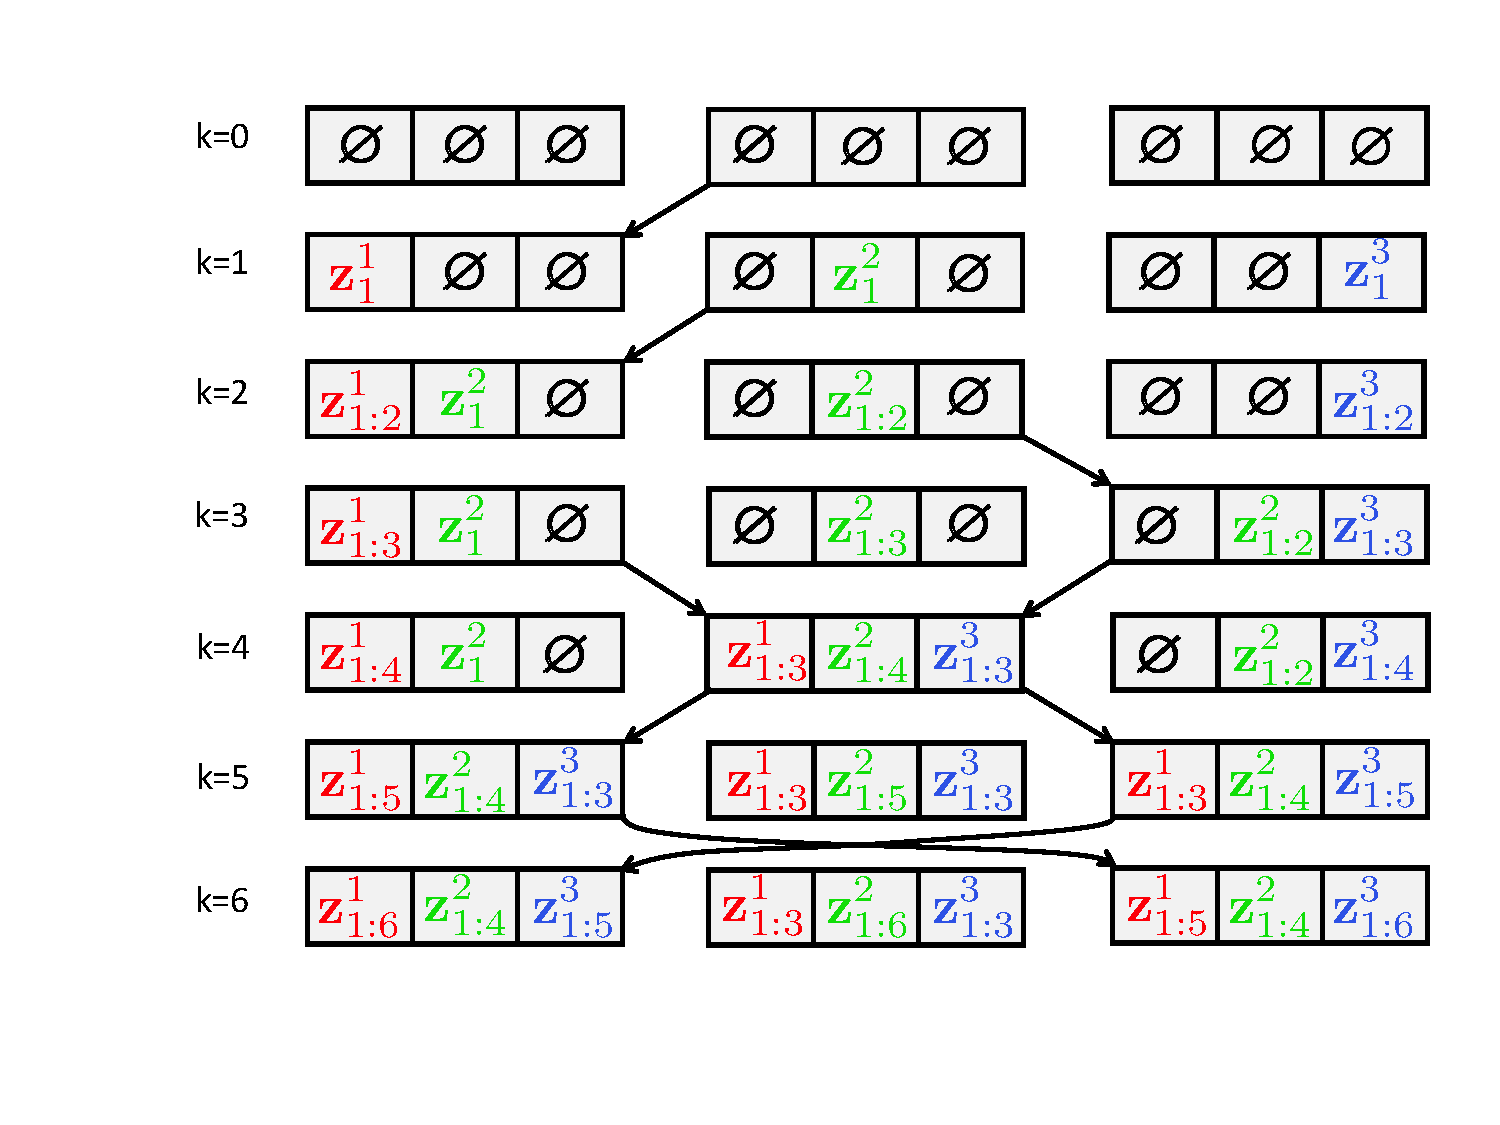
\includegraphics[width=0.5\textwidth]{figures/fifo}
		\caption{Example of {\proto} with three UGVs under dynamically changing interaction topologies. The arrows represent a directed communication link between two UGVs. $\varnothing$ denotes the empty set. For the purpose of clarity, we only show measurements, not the states, in the CB in this example.}
		\label{fig:\proto}
		%		\vspace{-1em}]
	\end{figure}		
	\section{Distributed Bayesian Filter via FIFO Protocol}\label{sec:\proto-dbf}
	We first introduce the generic distributed Bayesian filter (DBF).
	%, which is also stated in \cite{bandyopadhyay2014distributed} and \cite{julian2012distributed}. 
	%Each UGV has its individual estimation of the probability density function (PDF) of target position, called \textit{individual PDF}. 
	Let $\X_k\in S$ be the random variable representing the position of the target at time $k$.
	Define $\Z^i_k$ as the set of measurements of time $k$ that are in the $i\thi$ UGV's CB, i.e., \small$\Z^i_k=\lb z^j_k| \left[x^j_k,z^j_k\right]\in \B^i_k,\; \forall j\in V\rb$\normalsize and let $\Z^i_{1:k} = \bigcup\limits_{t=1}^k \Z^i_t$. 
	We also define $z^i_{1:k}=\left[z^i_1,\dots,z^i_k\right]$ as the set of the $i\thi$ UGV's measurements of times $1$ through $k$.
%	\todohere{probably use $z^V_{1:k}$ here? And then use $z^i_{1:k}$ as the set for only UGV $i$.}
	The probability density function (PDF) of $\X_k$, called \textit{individual PDF}, of the $i\thi$ UGV is represented by
	%=\left\lbrace z^i_1,\dots,z^i_k\right\rbrace
	$P^i_{pdf}(\X_{k}|\Z^i_{1:k})$.
	It is the estimation of the target position given all the measurements that the $i\thi$ UGV has received.	
%	where $\mathbf{z}^i_{1:k}$ denotes the set of measurements by $i\thi$ UGV and by UGVs in $\mathcal{Q}_i$, that have been received by $i\thi$ UGV until time $k$.
	%by UGVs in $\mathcal{Q}_i$ that have been transmitted to $i\thi$ UGV by time $k$.
	%from time $1$ through $k$ and $z^{\mathcal{Q}_i}_{1:k}$ means the set of measurements by UGVs in $\mathcal{Q}_i$ that are transmitted to $i\thi$ UGV.
	%Note that if the measurement by $j\thi(j\in \mathcal{Q}_i)$ UGV at time $k'(k'\leq k)$ is not received by $i\thi$ UGV, the corresponding element $z^j_{k'}$ in $z^{\mathcal{Q}_i}_{1:k}$ is empty and thus not utilized for computing $i\thi$ individual PDF.
	The initial individual PDF, $P^i_{pdf}(\X_0)$, is constructed %=P(\X_0) $P^i_{pdf}(\X_0|\mathbf{z}^i_0)$
	%$P^i_{pdf}(x_0|z^i_0,z^{\mathcal{Q}_i}_0)=P(x_0)$, 
	given prior information including past experience and environment knowledge. 
	It is necessary to initialize $P^i_{pdf}(\X_0)$ such that the probability density of the true target position is nonzero, i.e., $P^i_{pdf}(\X_0=x^g_0)> 0$.
	
	Under the framework of DBF, the individual PDF is recursively estimated by two steps: the prediction step and the updating step. 
	%, based on measurements of $i\thi$ UGV and UGVs in $\mathcal{Q}_i$.
	
%	\subsubsection{Prediction}
	%The $i\thi$ individual PDF at time $k-1$ is known, denoted as $P^i_{pdf}(x_{k-1}|z^i_{1:k-1},z^{\mathcal{Q}_i}_{1:k-1})$. 
	%At time $k$, the prior individual PDF $P^i_{pdf}(x_{k-1}|z^i_{1:k-1},z^{\mathcal{Q}_i}_{1:k-1})$ is first predicted forward by using the Chapman-Kolmogorov equation:
	\textbf{Prediction.}
	At time $k$, the prior individual PDF $P^i_{pdf}(\X_{k-1}|\Z^i_{1:k-1})$ is first predicted forward by using the Chapman-Kolmogorov equation:
	%\small\begin{align}\label{eqn:bayes_pred}
	%&P^i_{pdf}(x_k|z^i_{1:k-1},z^{\mathcal{Q}_i}_{1:k-1})\notag\\
	%&=\int P(x_k|x_{k-1})P^i_{pdf}(x_{k-1}|z^i_{1:k-1},z^{\mathcal{Q}_i}_{1:k-1})dx_{k-1}
	%\end{align}\normalsize
	\small
	\begin{equation}\label{eqn:bayes_pred}
	P^i_{pdf}(\X_k|\Z^i_{1:k-1})
	=\int\limits_{\X_{k-1}\in S} P(\X_k|\X_{k-1})P^i_{pdf}(\X_{k-1}|\Z^i_{1:k-1})d\X_{k-1},
	\end{equation}\normalsize
	where $P(\X_k|\X_{k-1})$ represents the state transition probability of the target, based on the Markovian motion model (\Cref{eqn:tar_motion_model}). % from the prior position $\X_{k-1}$ to the posterior position $\X_k$, 
	% independent of UGV states. 
	%This model describes 
	%Note that the target is static in many search applications, such as the indoor search for stationary objects \cite{kulich2014single}. 
	%, as defined in \Cref{eqn:tar_motion_model},
%	For the deterministic motion model, the state transition probability is simplified to be
%	\small\begin{equation}\label{eqn:markov_model}
%	P(\X_k=c_k|\X_{k-1}=c_{k-1})=\begin{cases}
%	1 & \text{if}\quad c_k=f(c_{k-1})\\ %
%	0 & \text{otherwise}
%	\end{cases}.
%	\end{equation}\normalsize
	
%	\subsubsection{Updating}
	\textbf{Updating.}
	The $i\thi$ individual PDF is then updated by the Bayes' rule using the set of newly received measurements at time $k$, i.e., $\Z^i_k$:
%	\small \begin{equation}
%	P^i_{pdf}(\X_k|\Z^i_{1:k})= K_iP^i_{pdf}(\X_k|\Z^i_{1:k-1})P(\Z^i_k|\X_k)
%	\end{equation}\normalsize
	\begin{subequations}\label{eqn:bayes_upd}
		\small\begin{align}
%			\begin{split}
				P^i_{pdf}(\X_k|\Z^i_{1:k})
				&= K_iP^i_{pdf}(\X_k|\Z^i_{1:k-1})P(\Z^i_k|\X_k)\label{subeqn:bayes_upd_general}\\
				&=K_iP^i_{pdf}(\X_k|\Z^i_{1:k-1})\prod\limits_{z^j_k\in\Z^i_k}P(z^j_k|\X_{k})\label{subeqn:bayes_upd_factor},
%			\end{split}
		\end{align}\normalsize
	\end{subequations}
	where $P(z^j_k|\X_k)$ is the sensor model and $K_i$ is a normalization factor, given by:
	\small\begin{align*}
	K_i=\left[\int\limits_{\X_k\in S} P^i_{pdf}(\X_k|\Z^i_{1:k-1})P(\Z^i_k|\X_k)d\X_k\right]^{-1}.
	\end{align*}\normalsize
	\textcolor{orange}{Here we have utilized the commonly adopted assumption \cite{furukawa2006recursive,gu2007distributed,sheng2005distributed} in the distributed filtering literature that the measurements of each UGV at current time are conditionally independent from its own previous measurements and the measurements of other UGVs given the target and the UGVs' current positions.
	This assumption allows us to simplify $P(\Z^i_k|\X_k,\Z^i_{1:k-1})$ as $P(\Z^i_k|\X_k)$ in \Cref{subeqn:bayes_upd_general} and factorize $P(\Z^i_k|\X_k)$ as $\prod\limits_{z^j_k\in\Z^i_k}P(z^j_k|\X_{k})$ in \Cref{subeqn:bayes_upd_factor}.}
%	The factorization of $P(\Z^i_k|\X_k)$ comes from the conditional independence of measurements from each UGV given the target position and the corresponding UGV's position.	
	
	\begin{algorithm}
		\caption{\proto-DBF Algorithm}\label{alg:lifo-dbf}
		\begin{algorithmic}
			\State For $i\thi$ UGV at $k\thi$ step ($\forall i\in V$):
			%				\State After the updating step in \cref{alg:lifo},
			\State\textbf{(1)} Initialize a \textit{temporary PDF} by assigning the stored individual PDF to it:
			\small\begin{equation*}
			P^i_{tmp}(\X_{t})= P^i_{sto}(\X_t),
			%			P^i_{pdf}(\X_{k-N}|z^1_{1:k-N},\dots,z^N_{1:k-N}).
			\end{equation*}\normalsize		
			where % the stored individual PDF is for time $t$:
			\small\begin{equation*}
			P^i_{sto}(\X_t) = P^i_{pdf}(\X_{t}|z^1_{1:t},\dots,z^N_{1:t}).
			\end{equation*}\normalsize	
			\State\textbf{(2)} For $\xi=t+1$ to $k$, iteratively repeat two steps of Bayesian filtering:
			
			\State(2.1) Prediction 
			\small\begin{equation*}
			P_{tmp}^{pre}(\X_{\xi})=\int_{S} P(\X_{\xi}|\X_{\xi-1})P^i_{tmp}(\X_{\xi-1})d\X_{\xi-1}.
			\end{equation*} \normalsize
			
			\State(2.2) Updating
			%				\small\begin{gather*}
			%				P^i_{tmp}(\X_{\xi})=K_{\xi} P_{tmp}^{pre}(\X_{\xi})\prod\limits_{j\in\Omega^i_{\xi}}P(z^j_{\xi}|\X_{\xi}),\\
			%				K_{\xi}=\left[\int_S P_{tmp}^{pre}(\X_{\xi})\prod\limits_{j\in\Omega^i_{\xi}}P(z^j_{\xi}|\X_{\xi})d\X_{\xi}\right]^{-1}.
			%				\end{gather*} \normalsize
			\small\begin{gather*}
			P^i_{tmp}(\X_{\xi})=K_{\xi} P_{tmp}^{pre}(\X_{\xi})P(\Z^i_{\xi}|\X_{\xi}),\\
			K_{\xi}=\left[\int_S P_{tmp}^{pre}(\X_{\xi})P(\Z^i_{\xi}|\X_{\xi})d\X_{\xi}\right]^{-1}.
			\end{gather*} \normalsize
			
			\State(2.3)
			If $z^j_{\xi}\neq\emptyset$ for $\forall j\in V$, update the stored PDF:
			%				When $\xi=t+1$, if $z^j_{t+1}\neq\emptyset$ for $\forall j\in V$, update the stored PDF:
			%				then the stored PDF will be updated to be the temporary PDF of time $t+1$:
			\small\begin{equation*}
			P^i_{sto}(\X_{\xi})=P^i_{tmp}(\X_{\xi}).
			%		P^i_{pdf}(\X_{k-N+1}|z^1_{1:k-N+1},\dots,z^N_{1:k-N+1})=P^i_{tmp}(\X_{k-N+1}).
			\end{equation*}\normalsize
			%				where 
			%				\small\begin{equation*}
			%				P^i_{tmp}(\X_{t+1})=P^i_{pdf}(\X_{t+1}|z^1_{1:t+1},\dots,z^N_{1:t+1}).
			%				\end{equation*}\normalsize
			
			\State\textbf{(3)} The individual PDF of $i\thi$ UGV at time $k$ is
			$P^i_{pdf}(\X_{k}|\Z^{i}_{1:k})=P^i_{tmp}(\X_k)$.		
		\end{algorithmic}
	\end{algorithm}
	
	\subsection{The FIFO-DBF Algorithm}
	The generic DBF is not directly applicable to time-varying interaction topologies. 
	This is because changing topologies can cause intermittent and out-of-sequence arrival of measurements from different UGVs, giving rise to the OOSM problem.
	One possible solution is to ignore all measurements that are out of the temporal order.
	This is undesirable since this will cause significant information loss.
	Another possible remedy is to fuse all measurements by running the filtering algorithm from the beginning at each time step.
	This solution naturally causes excessive computational burden.
	To avoid both OOSM problem and unnecessary computational complexity, we add a new PDF, namely the \textit{stored PDF}, $P^{i}_{sto}(\X_t)$, that is updated from the $i\thi$ UGV's initial PDF by fusing the state-measurement pairs of \textit{all} UGVs up to a certain time $t\le k$.
	The choice of $t$ is described in \Cref{subsec:tracklist}.
	%	 that are in the $i\thi$ UGV's CB.	
	%	Therefore, the choice of $t$ needs to ensure that the $i\thi$ UGV has received the state-measurement pairs of times no greater than $t$ from all UGVs, which is described in \Cref{sec:tracklist} by using the track lists.
	The individual PDF, $P^i_{pdf}(\X_k|\Z^i_{1:k})$, is then computed by fusing the measurements from time $t+1$ to $k$ in the CB into $P^i_{sto}(\X_t)$, running the Bayesian filter (\Cref{eqn:bayes_pred,eqn:bayes_upd}).
	Note that initially, $P^{i}_{sto}(\X_0)$ = $P^i_{pdf}(\X_0)$.
	
	The \textbf{\proto-DBF algorithm} is stated in \cref{alg:lifo-dbf}.
	Each UGV runs \proto-DBF after its CB is updated in the Updating Step in \Cref{alg:lifo}.
	At the beginning, we assign the stored PDF to a temporary PDF, which will then be updated by sequentially fusing measurements in the CB to obtain the individual PDF.
	%	We use $\Omega^i_{\xi}\,\left(\xi=t+1,\dots,k\right)$ to denote the index set of UGVs whose state-measurement pair of time $(\xi)$ is stored in $i\thi$ UGV's CB, i.e. $\Omega^i_{\xi}=\left\lbrace j\in \mathcal{Q}_i \bigcup \left\lbrace i \right\rbrace | \left[x^j_\xi,z^j_{\xi}\right]\in B^i_k\rb$.
	%	The measurements will be sequentially used to update the temporary PDF until the latest measurements are used.
%	The temporary PDF is then assigned as the individual PDF of time $k$.
	It should be noted that, when the UGV's CB contains all UGVs' state-measurement pairs from $t$ to $\xi$, the temporary PDF of $\xi$ is assigned as the stored PDF.
	\cref{fig:LIFO-DBF} illustrates the \proto-DBF procedure for the $1^\text{st}$ UGV as an example.
	It can be noticed that, the purpose of using the stored PDF is to avoid running the Bayesian filtering from the initial PDF at every time step. 
	Since the stored PDF has incorporated all UGVs' measurements up to some time step $t$, the information loss is prevented. % when computing the individual PDF.
	%	each UGV only needs to start from the stored PDF each time it computes the individual PDF.
	We point out that the time $t$ of each UGV's stored PDF can be different from others.
	The stored PDF is saved locally by each UGV and not transmitted to others.
%	\footnote{\todohere{change notations here} Due to the space limit, in this figure we use $P^i_{pdf}(k)$, $P^i_{pdf}(k-N)$ and $P^i_{pdf}(k-N+1)$ to represent $P^i_{pdf}(\X|\mathbf{z}^{i}_{1:k})$ $P^i_{pdf}(\X|\mathbf{z}^{i}_{1:k-N})$ and $P^i_{pdf}(\X|\mathbf{z}^{i}_{1:k-N+1})$, respectively.}.
	
	\begin{figure}%[thpb]
		\centering
		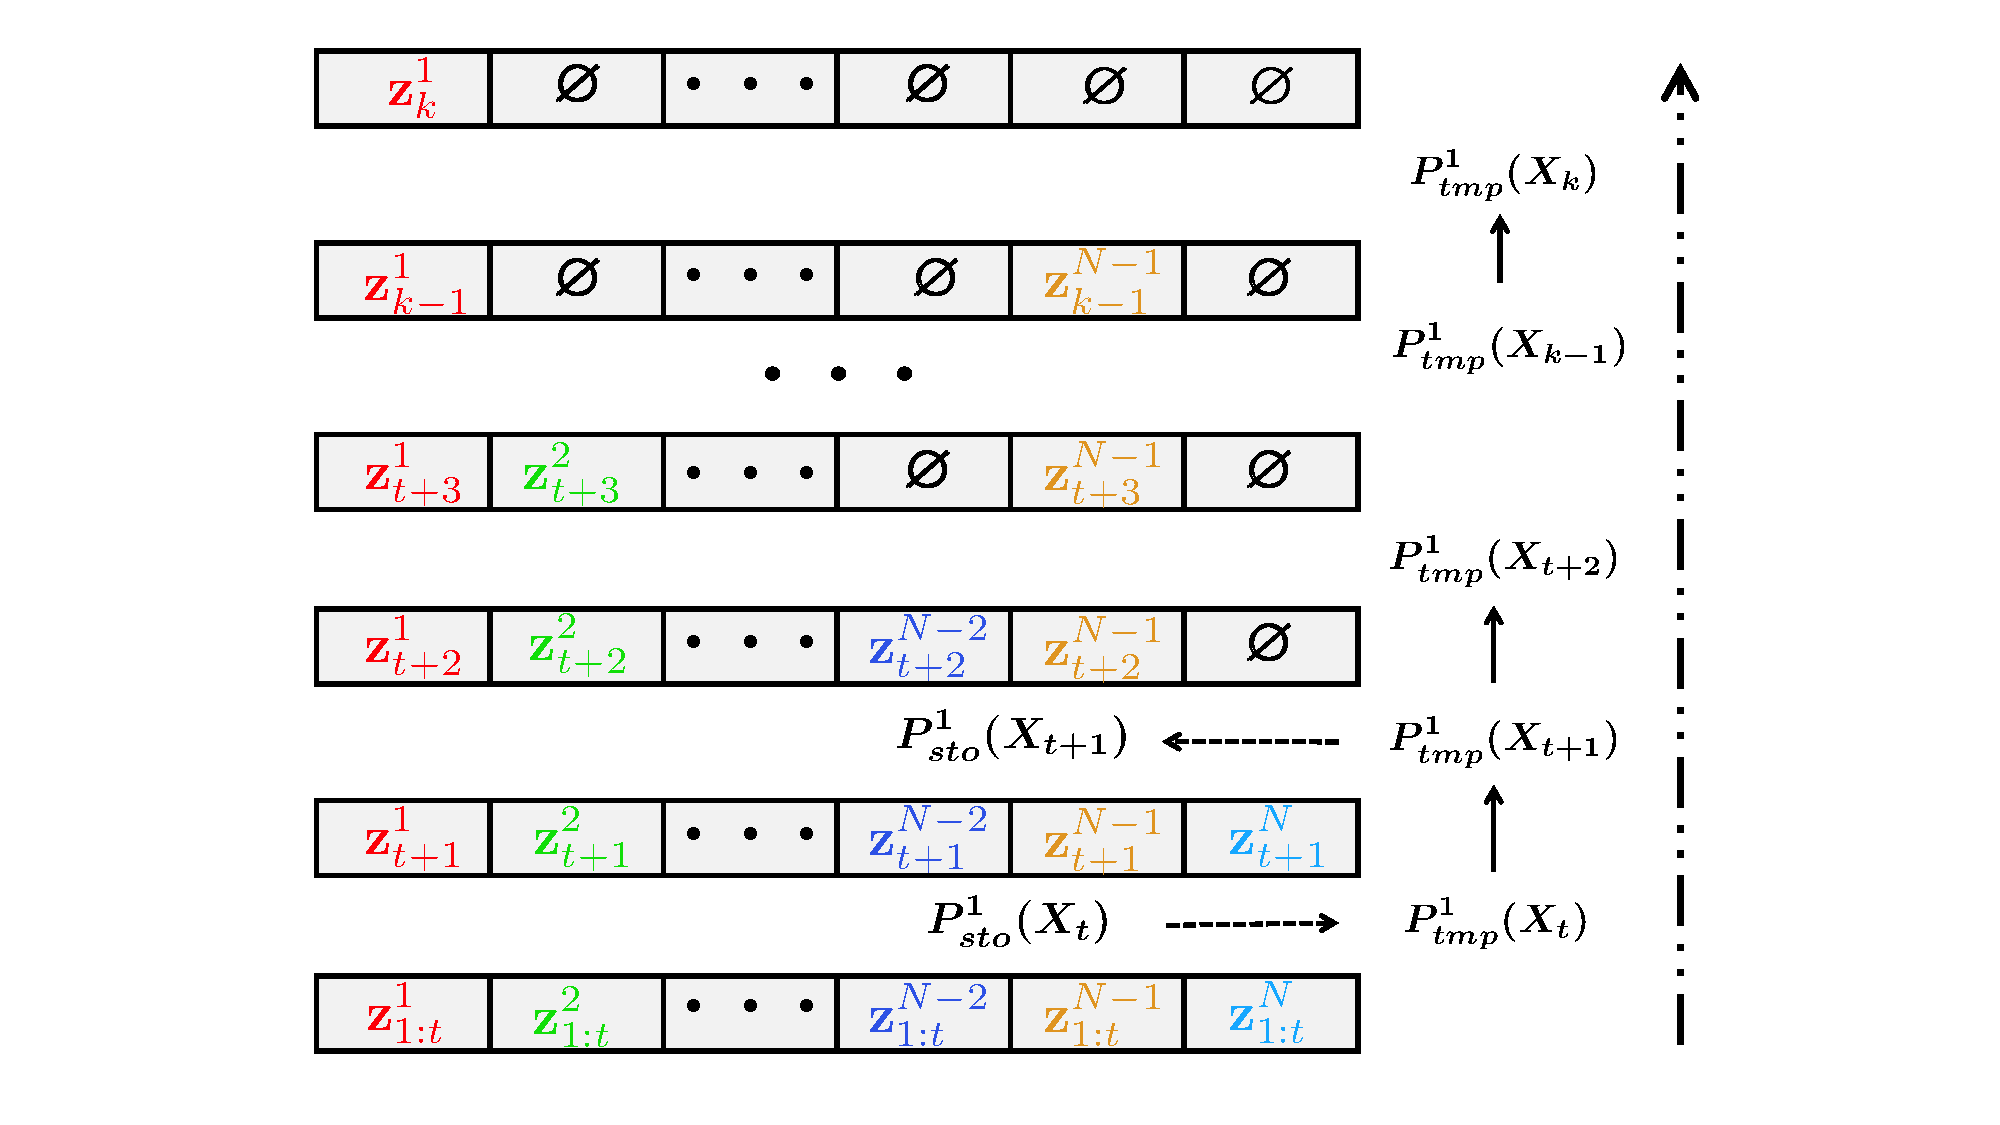
\includegraphics[width=0.50\textwidth]{figures/fifo-dbf}
		\caption{Example of \proto-DBF for the $1^\text{st}$ UGV at time $k$. 
			Only the measurement (not the state) is shown in the figure.
%			Networked UGVs take a line topology.
%			The stored individual PDF is represented by $ P^1_{pdf}(k-N)$.
			The UGV first calculates $ P^1_{tmp}(X_{t+1})$. 
			Since the UGV has received all UGVs' measurements of $t+1$, the $ P^1_{tmp}(X_{t+1})$ is assigned as the new stored PDF. 
			The dashed arrow on the right shows the order to fuse measurements in the CB.}
%			Repeating DBF until obtaining $ P^1_{pdf}(k)$.
			%		, which is the individual PDF at time $k$.
%			In this example, $\Omega^1_{\xi}=\left\lbrace 1,2,\dots,N+1-\xi\right\rbrace $, $\xi=1,\dots,N$.}
		\label{fig:LIFO-DBF}
%		\vspace{-1em}
	\end{figure}			
	
	\subsection{Track Lists for Trimming CBs}\label{subsec:tracklist}
	
	\begin{algorithm}
		\caption{Updating TLs}
		\label{alg:upd_tl}
		\begin{algorithmic}
			\State Consider updating the $i\thi$ UGV's TL, $\Q^i_k$, using the received $r\thi$ UGV's TL, $\Q^r_{k-1}(r\in \N^\text{in}_i(G_{k-1}))$.		
			\State \textbf{(1)} Update the $i\thi$ row of $\Q^i_k$, using $\B^i_k$:
			\begin{itemize}
				\item choose $k^{ii}$ as the minimum integer that satisfies the following conditions: (a) $\exists l\in V \text{ s.t. } \left[x^l_{k^{ii}},z^l_{k^{ii}}\right]\notin \B^i_k$ and (b) $k^{ii} \ge t_m-1$, where $t_m$ is the minimum time of state-measurement pairs in $\B^i_k$.
			\end{itemize}
			\State \textbf{(2)} Update other rows of $\Q^i_k$:
			$\forall j\in V\setminus\lb i\rb$
			\begin{itemize} 
				\item if $k^{ij}>k^{rj}$, keep current $\mathbf{q}^{ij}_{k^{ij}}$;
				\item if $k^{ij}=k^{rj}$, $\mathbf{q}^{ij}_{k^{ij}}=\mathbf{q}^{ij}_{k^{ij}} \lor\footnotemark\mathbf{q}^{rj}_{k^{rj}}$; 
				\item if $k^{ij}<k^{rj}$, $\mathbf{q}^{ij}_{k^{ij}}=\mathbf{q}^{rj}_{k^{rj}}$ and $k^{ij}=k^{rj}$.
			\end{itemize}
		\end{algorithmic}
	\end{algorithm}
	\footnotetext{`$\lor$' is the notation of the logical `OR' operator.}
	
	\begin{figure}%[thpb]
		\centering
		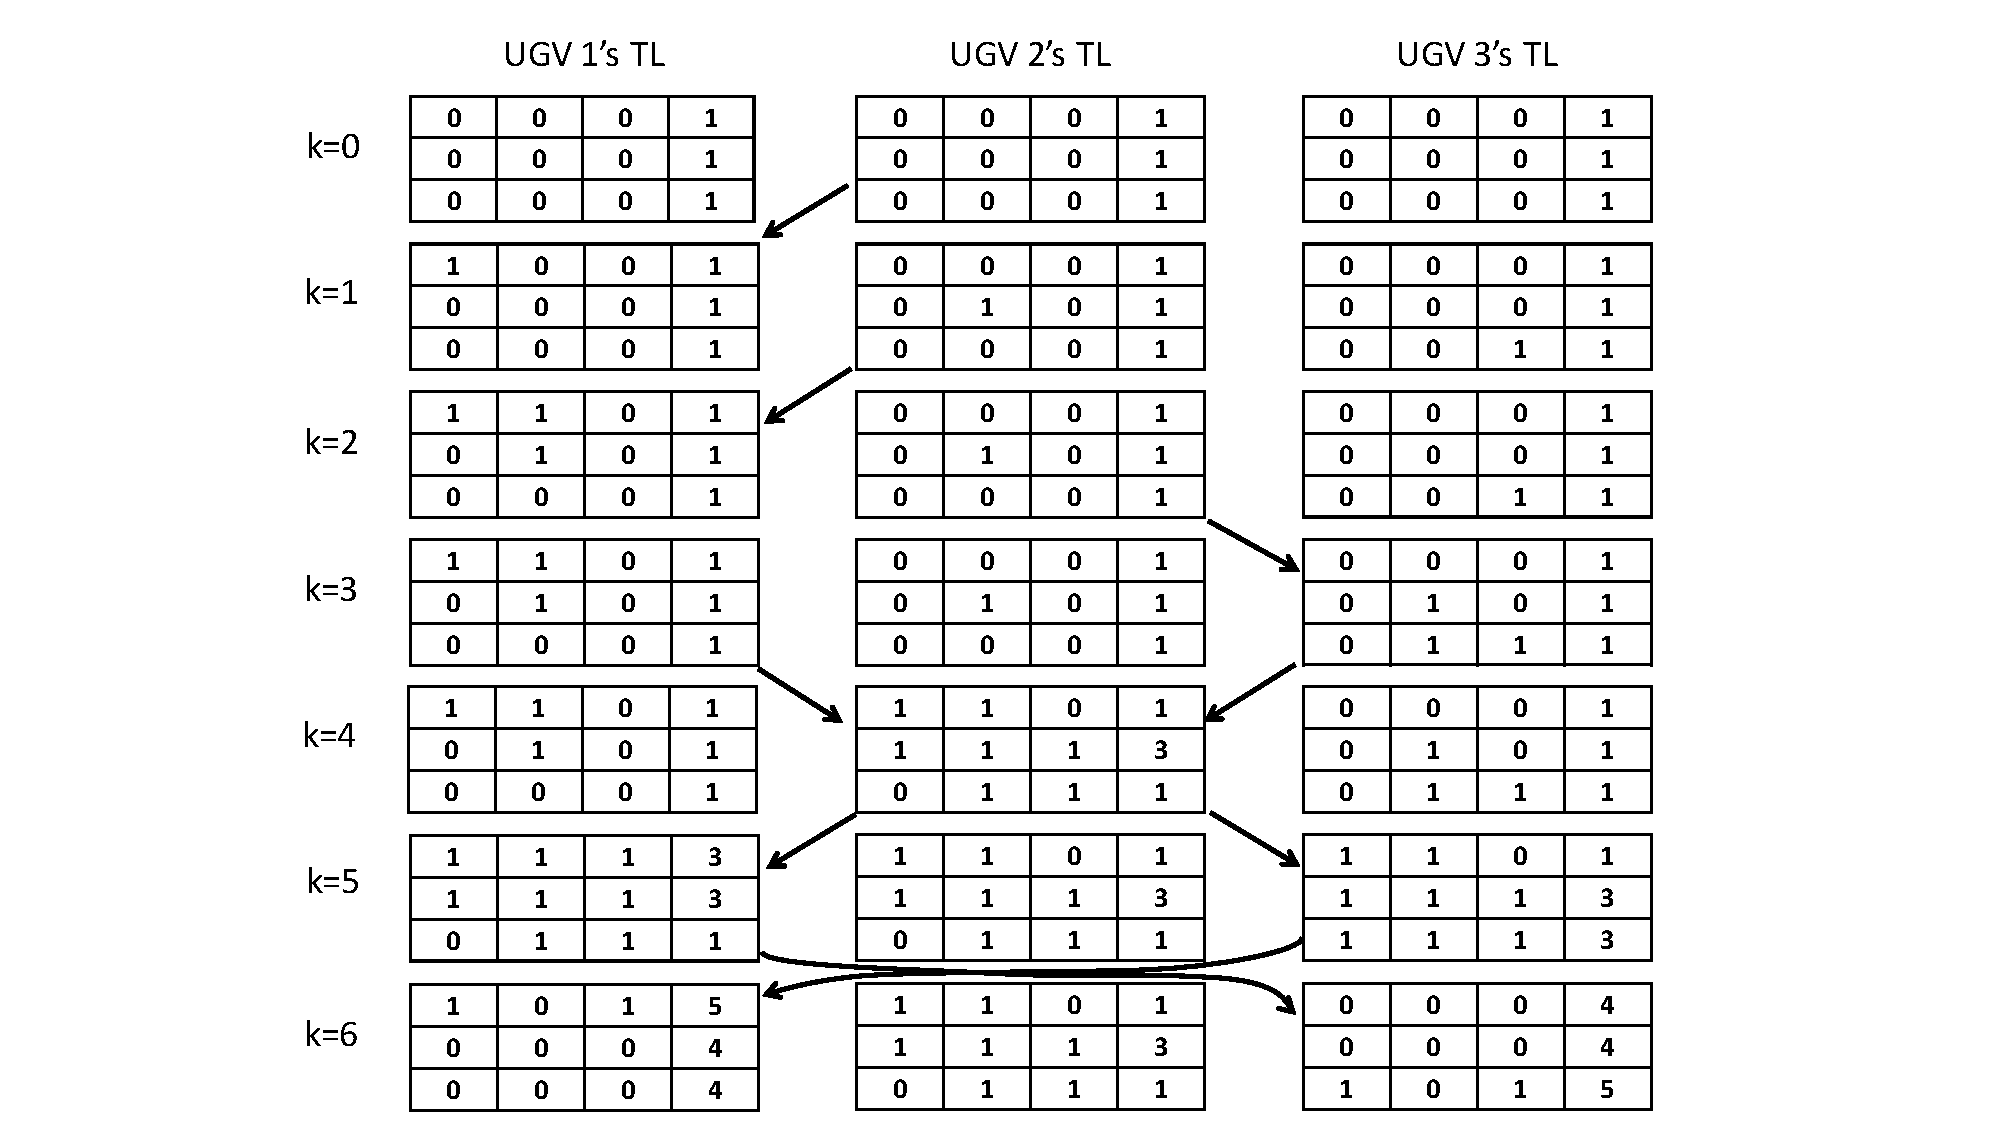
\includegraphics[width=0.50\textwidth]{figures/track_list}
		\caption{Example of updating TLs. For the $1^\text{st}$ UGV's TL, the $j\thi\,(j\in V)$ entry on the $i\thi\,(i\in V)$ row represents this UGV's knowledge about whether the $i\thi$ UGV has received the $j\thi$ UGV's state-measurement pair of time $k^{1i}$, where $k^{1i}$ is the last entry of the $i\thi$ row. TLs are updated using \cref{alg:upd_tl,alg:tracklist}.}
		\label{fig:upd_tl}
%		\vspace{-1em}
	\end{figure}
	
	The size of CBs can keep increasing as measurements cumulate over time. 
	The use of the stored PDF has made it feasible to trim excessive measurements from the CBs.
	%	while ensuring no information is lost in the sense that all UGVs' measurements have been used for update hte individual PDF.
	To avoid information loss, a state-measurement pair can only be trimmed from a UGV's CB when \textit{all} UGVs have received it.
	To keep track of each UGV's reception of other UGVs' measurements, every UGV maintains a \textit{track list} (TL), $\Q^i_k=\left[\mathbf{q}^{i1}_{k^{i1}},\dots, \mathbf{q}^{iN}_{k^{iN}}\right]^T \,(\forall i\in V)$, where $\mathbf{q}^{ij}_{k^{ij}}=\left[q^{j1}_{k^{ij}},\dots,q^{jN}_{k^{ij}},k^{ij}\right]^T$ ($j\in V$) is a $(N+1)\times 1$ binary vector.
	Therefore, a TL can be represented by a binary matrix of size $N\times (N+1)$, with the last column corresponding to the measurement time.
	$\Q^i_k$ represents the $i\thi$ UGV's knowledge of its own and other UGVs' measurements of the times specified by $k^{ij}\,(j\in V)$: %, in terms of the measurement time,
	the entry $q^{jl}_{k^{ij}}$ equals $1$ if the $i\thi$ robot knows that the $j\thi$ UGV has received the state-measurement pair of the $l\thi$ UGV of time $k^{ij}$, $\left[x^l_{k^{ij}},z^l_{k^{ij}}\right]$, and equals $0$ if the $i\thi$ robot cannot determine whether $\left[x^l_{k^{ij}},z^l_{k^{ij}}\right]$ has been received by the $j\thi$ robot, i.e.,
	%	\begin{equation*}
	%	q^{j,l}_{k^{j}}=
	%	\begin{cases}
	%	1 & \text{if}\quad \exists t\in\mathbb{N}, \text{ s.t. }k^{i,j}\le t\le k \text{ and } \left[x^l_{k^{i,j}},z^l_{k^{i,j}}\right]\in B^j_t,\\
	%	0 & \text{if}\quad \nexists t\in\mathbb{N}, \text{ s.t. }k^{i,j}\le t\le k \text{ and } \left[x^l_{k^{i,j}},z^l_{k^{i,j}}\right]\in B^j_t.
	%	\end{cases}
	%	\end{equation*}
	\small\begin{equation}\label{eqn:tl_entry}
	q^{jl}_{k^{ij}}=
	\begin{cases}
	1 & \text{if}\quad \exists t\in\left[k^{ij}, k\right] \text{ s.t. } \left[x^l_{k^{ij}},z^l_{k^{ij}}\right]\in \B^j_t,\\
	0 & \text{if}\quad \nexists t\in\left[k^{ij}, k\right] \text{ s.t. } \left[x^l_{k^{ij}},z^l_{k^{ij}}\right]\in \B^j_t.
	\end{cases}
	\end{equation}\normalsize
	Therefore it can happen that $\left[x^l_{k^{ij}},z^l_{k^{ij}}\right]$ has been received by the $j\thi$ UGV but the $i\thi$ UGV does not know this and thus $q^{jl}_{k^{ij}}=0$.
	
%	When all elements of $\Q^i_k$ are $1$'s, the $i\thi$ UGV can be sure that the $j\thi$ UGV ($\forall j\in V$) has received the state-measurement pairs of time $k^{i,j}$ from all UGVs.
	%	Choose the minimum time $k^i_m=\min\limits_j k^{i,j}$.
	%	Then the $i\thi$ robot fuse all the measurements of time no greater than $k^i_m$ in its own CB to update the stored PDF.
	%	TLs are exchanged when UGVs communicate and are used to trim the CBs. 
%	\todohere{rethink about how many steps a TL can be trimmed.}
	
	The exchange and updating of TLs are described in \Cref{alg:lifo}, with the updating details presented in \cref{alg:upd_tl}.
	For the $i\thi$ UGV, it updates the $i\thi$ row of its TL matrix using the entries of its CB, and updates other rows of the TL using the received TLs from {\inbhd}.
	The updating rule guarantees that, if the last term of the $j\thi$ row is $k^{ij}$, the $i\thi$ UGV is ensured that every UGV has received state-measurement pairs of times earlier than $k^{ij}$ from all UGVs.
	The \Cref{alg:tracklist} describes the approach to trim CBs using TLs.
%	Note that, due to the trimming of CBs, (2.3) in \Cref{alg:lifo-dbf} needs to be revised as follows:
%	
%	If $\xi<k^i_m$, then update the stored PDF:
%	\small\begin{equation*}
%	P^i_{sto}(\X_{\xi})=P^i_{tmp}(\X_{\xi}).
%	%		P^i_{pdf}(\X_{k-N+1}|z^1_{1:k-N+1},\dots,z^N_{1:k-N+1})=P^i_{tmp}(\X_{k-N+1}).
%	\end{equation*}\normalsize	
%	Since a TL only keeps track of the earliest measurements in CBs, the CBs are only trimmed by one time step each time the trim happens.
	\cref{fig:upd_tl} shows the updating of each UGV's TLs using the \cref{alg:upd_tl}.
	In the example, the $1^\text{st}$ and $3^\text{rd}$ UGV's CB will be trimmed at $k=6$ and the trimmed state-measurement pairs corresponds to times $1,2,$ and $3$.
	
	The use of TLs can avoid the excessive size of CBs and guarantee that trimming the CBs will not lose any information; the trimmed measurements have been encoded into the stored PDF.
	The following theorem formalizes this property.
	
	\begin{thm}\label{thm:trim_no_loss}
%		For a {\fc} network using FIFO-DBF, 
%		each UGV's individual PDF is updated with measurements from all UGVs. 
		Each UGV's estimation result using the trimmed CB is the same as that using the non-trimmed CB.
	\end{thm}
	
	\begin{proof}
%		According to \Cref{cor1}, each UGV receives the state-measurement pairs from all other UGVs within finite time steps that are used for updating the individual PDF.
		
		Consider the $i\thi$ UGV. Let $k^i_m=\min\limits_j k^{ij}$. 
		Trimming $\B^i_k$ happens when all entries in $\Q^i_k$ corresponding to time $k^i_m$ equal $1$. 
		This indicates that each UGV has received the state-measurement pairs of time $k^i_m$ from all UGVs.
%		, i.e., $\left[x^l_{k_m},z^l_{k_m}\right],\,l\in V$. 
		A UGV has either stored the pairs in its CB or already fused them to obtain the stored PDF.
		In both cases, such pairs are no longer needed to be transmitted. %since it will not add any unused information to the multi-agent team. 
		Therefore, it causes no loss to trim theses measurements.		
%		\hfill\qedsymbol
	\end{proof}
	
	%	Since TLs are used to reduce the size of CBs, it is necessary to understand how often the CBs will be trimmed.
%	The following theorem describes when CBs get trimmed.
	\textcolor{orange}{The following theorem describes when CBs get trimmed, and it provides an upper bound of the communication burden that FIFO will incur.
	A detailed complexity analysis of FIFO-DBF is presented in \Cref{subsec:complexity}.}
	Consider trimming all the state-measurement pairs of time $t$ in the $i\thi$ UGV's CB.
	Let $k^{lj}_t (>t)$ be the first time that the $l\thi$ UGV communicates to the $j\thi$ UGV in the time interval $(t,\infty)$.
	Define $\tilde{k}^j_t=\max\limits_l k^{lj}_t$, which is the time that the $j\thi$ UGV receives all other UGVs' measurements of $t$.
	Similarly, let $k^{ji}_t (> \tilde{k}^j_t)$ be the first time that the $j\thi$ UGV communicates to the $i\thi$ UGV in the time interval $(\tilde{k}^j_t,\infty)$ and define $\tilde{k}^i_t=\max\limits_j k^{ji}_t$.
	%	Let $d_{ji}$ is the shortest path distance from UGV $j$ to $i$ in the time interval $[t+d_{lj},t+d_{lj}+d_{ji}]$. 
	The following theorem gives the time when the $i\thi$ UGV ($\forall i\in V$) trims all state-measurement pairs of time $t$ in its own CB.
	\begin{thm}\label{thm:upd_tl_freq}		
		The $i\thi$ UGV trims $\lb\left[x^l_t,z^l_t\right] \,(\forall l\in V)\rb$ from its CB at the time $\tilde{k}^i_t$.
		%		interval $[\tilde{k}^i_t,t+2(N-1)T_u]$.
	\end{thm}
	
	\begin{proof}
%		We consider the case when the lower bound is achieved.
%		Assume that at time $t$ after the updating step, each UGV's CB only contains its own state-measurement pair of time $t$.
%		Then at $\tilde{k}_j$, the $j\thi$ UGV's CB has received all other UGVs' measurements at $t$.
		The $i\thi$ UGV can trim $\lb\left[x^l_t,z^l_t\right] \,(\forall l\in V)\rb$ only when it is sure that all other UGVs have also received these state-measurement pairs.
		This happens at $\tilde{k}^i_t$ and is thus the time when the trim occurs. 
		
%		\hfill\qedsymbol
		
		%		To compute the upper bound, we consider the time interval between the trims of time $t$ and $t+1$.\part{title}
		%		The largest interval is achieved when the CBs of all UGVs at $t$ are all empty
		
		%		The first time for the $j\thi$ UGV to receive $B^l_t$ from $l\thi$ UGV is time $t_{lj}$ and the $j\thi$ UGV's TL is updated so that $q^{j,l}_{t'}=1$ for some $t'\le t$.
		%		If $t'=t$, then all measurements before $t$ from the $l\thi$ UGV has already been fused to generate $P^j_{sto}(\X_{t-1})$. 
		%%		This is the case thus the shortest possible time to trim all the state-measurement pairs of $t$ in $i\thi$ UGV's CB.
		%		The first time the $i\thi$ UGV knows $g^{j,l}_{t'}=1$ is at time $k^{lji}_t$, when the $j\thi$ UGV's TL is transmitted to $i\thi$ UGV.
		%		Therefore, $\max\limits_{l,j\in V} k^{lji}_t$ is the earliest time when the $i\thi$ UGVs know about each UGV's reception of all measurements of time $t$.
		%				
		%		If $i\thi$ UGV's stored PDF corresponds to the time step $t-1$, then the trim happens at $k^i_t= \max\limits_{l,j\in V} k_t^{lji}$.
		%		If the stored PDF corresponds to a time step less than $t-1$, then the trim happens at $k^i_t> \max\limits_{l,j\in V} k_t^{lji}$.
		%		Therefore $k^i_t\ge \max\limits_{l,j\in V} k_t^{lji}$.
		%		The upper bound can be obtained using \Cref{prop1}.
	\end{proof}
	
	%	From \Cref{thm:upd_tl_freq}, we can get the following corollaries about how often the CB gets trimmed.
	
%	\begin{cor}
%		The first time to trim the $i\thi$ UGV's CB occurs at $\tilde{k}^i_1$.
%	\end{cor}
%	
%	\begin{proof}
%		%		The proof is straightforward by setting $t=1$ in the proof of \Cref{thm:upd_tl_freq} and 
%		Notice that the initial stored PDF of each UGV corresponds to the time $0$.
%		Therefore, the first time a TL is all $1$'s the trim occurs.
%	\end{proof}	
	
%	Under the \fc ness condition, the size of each UGV's CB is bounded.
%	\begin{thm}
%		The maximum interval between two consecutive trims is no greater than $T_M$.
%	\end{thm}
%	\begin{proof}
%		See the Appendix.
%	\end{proof}
	
	\begin{cor}\label{thm:max_CB_size}
		Under the \fc ness condition, the size of any UGV's CB is no greater than $2N(N-1)T_u$.
	\end{cor}
	
	\begin{proof}
		We consider an arbitrary $i\thi\,(i\in V)$ UGV.
		According to \Cref{prop1}, a UGV can communicate to any other UGV within $NT_u$ steps.
		Therefore, $\tilde{k}^i_t\le 2NT_u$, since it first requires each UGV communicate to all other UGVs and then each UGV communicate to the $i\thi$ UGV.
		This implies that, the state-measurement pairs of a certain time of all UGVs will be trimmed from each UGV's CB within $2NT_u$ steps.

		The maximum size the of CB occurs when the state-measurement pairs of a certain time from all but one UGV are saved in the $i\thi$ UGV's CB.
		Therefore, the size of any UGV's CB is no greater than $2N(N-1)T_u$.		
		
%		\hfill\qedsymbol
	\end{proof}
	
%	\begin{proof}
%		
%		Consider the time intervals $\left[k_m,k_{m+1} \right),\,m=1,2,\dots$ that are {\fc}, where $k_1=0$.
%		Define $\Delta_m = k_{m+1}-k_m,\,m=1,2,\dots$.
%		It is easy to know that $\Delta_i\le T_u$.
%		At $k_2$, the worst-case size of a UGV's CB is $(N-1)\Delta_1$.	
%		This can occur if UGVs do not communicate with each other until at $k_2$, when a UGV communicates with all others except one.
%		At $k_3$, according to the definition of a {\fc} network, every UGV has received measurements made at or before time $k_2$ from all UGVs.
%		The worst-case size of a UGV's CB is then $max \left[(N-1)(\Delta_2-\Delta_1),N(\Delta_1-\Delta_2)\right]$.  %$\Delta_2 = max(k_3-k_2-\Delta_1,0)$.
%		The first term is the worst-case size if $\Delta_2\ge\Delta_1$ and can be achieved similarly to the case of the time interval $\left[k_1,k_2\right)$. 
%		The second term corresponds to the worst-case size when $\Delta_1>\Delta_2$ and can be achieved if a UGV can receive measurements from all other UGVs in the whole time interval $\left[k_2,k_3\right)$. 
%		In general, at $k_{m+1}$, each UGV has already received all UGVs' measurements made at or before time $k_m$. 
%		The worst-case size of a UGV's CB within the time interval $\left[k_m,k_{m+1}\right)$ is $max\left[(N-1)(\Delta_m-\Delta_{m-1}),N(\Delta_{m-1}-\Delta_m)\right]$.
%		Since $\Delta_m\le T_u,\, m=1,2,\dots$, we know that the maximum CB size of each UGV is no greater than $NT_u$.
%	\end{proof}
	
	%	\begin{cor}
	%		The time between two consecutive trims of the $i\thi$ UGV's CB is 
	%		\begin{equation*}
	%			\Delta k_i=\begin{cases}
	%			1+n'_{i,t+1}-n_{i,t}& \text{if}\;n'_{i,t+1} \ge n_{i,t}\\
	%			1& \text{if}\;n'_{i,t+1} < n_{i,t}
	%			\end{cases},
	%		\end{equation*}
	%		where $n_{i,t}=\max\limits_{l,j}t_{ji}$ starting from $t$ and $n'_{i,t+1}=\max\limits_{l,j}t_{ji}$ starting from $t+1$.
	%	\end{cor}
	%	
	%	\begin{proof}
	%		Let $k_i = t+1+n_i$ and $k'_i = t+n'_i$ be the two consecutive trimming times.
	%		Since earlier measurements are always trimmed before the later measurements, this guarantees $\Delta k \ge 1$. 
	%		If $n'_i \ge n_i$, then it takes longer time for the later measurements to be trimmed and thus $\Delta k = 1+n_i'-n_i$.
	%	\end{proof}
	
	\begin{algorithm}
		\caption{Trimming CBs using TLs}
		\label{alg:tracklist}
		\begin{algorithmic}
			\State 
			For the $i\thi$ UGV:			
			find the smallest time in $\Q^i_k$: $k^i_m=\min\lb k^{i1},\dots,k^{iN} \rb$. 
			\begin{enumerate}
				\item Remove state-measurement pairs in $\B^i_k$ that corresponds to measurement times earlier than $k^i_m$, i.e., $\B^i_k=\B^i_k\setminus \lb\left[x^l_t,z^l_t\right] \rb,\,\forall t< k^i_m, \forall l\in V.$
				\item If entries associated with time $k^i_m$ in $\Q^i_k$ are $1$'s, then 
				\begin{enumerate}
					\item set these entries to be $0$.
					\item update the $i\thi$ row of $\Q^i_k$ using the current CB, i.e., $q^{il}_{k^{ij}}=1$ if $\left[x^l_{k^{ij}},z^l_{k^{ij}}\right]\in \B^i_k,\,\forall l\in V$.
					\item remove all corresponding state-measurement pairs in $\B^i_k$, i.e., $\B^i_k=\B^i_k\setminus \lb\left[x^l_{k^i_m},z^l_{k^i_m}\right] \rb,\, \forall l\in V.$
					\item $k^i_m \leftarrow k^i_m+1.$
				\end{enumerate}	
			\end{enumerate}				
		\end{algorithmic}
	\end{algorithm}
	
	\subsection{Complexity Analysis of FIFO-DBF}\label{subsec:complexity}
	Compared to statistics dissemination, {\proto} is usually more communication-efficient for distributed filtering. 
	To be specific, consider a grid representation of the environment with the size $D\times D$. %with a network of $N$ UGVs, 
	The transmitted data between each pair of UGVs are the CB and TL of each UGV.
	%	 and the corresponding UGV positions where observations were made, the length of which is $O(N)$. 
	The size of the CB is upper bounded by $O(N^2T_u)$, according to \Cref{thm:max_CB_size}.
%	$O(NT_M)$, according to \Cref{thm:max_CB_size}, and the size of the TL is $O(N^2)$.
%	Since $T_M\le (N-1)T_u)$, the overall communication complexity is upper bounded by $O(N^2T_u)$.	
	On the contrary, the communicated data of a statistics dissemination approach that transmits unparameterized posterior distributions or likelihood functions is $O(D^2)$.
	%	, which is in the order of environmental size. 
	In applications such as the target localization, $D$ is generally much larger than $N$ and the consensus filter usually requires multiple rounds to arrive at consensual results.
	Therefore, when $T_u$ is not comparable to $D^2$, the {\proto} protocol requires much less communication burden.
	
	%	It is worth noting that, for the static target, each UGV only needs current-step CB to update individual PDFs. 
	%	Therefore, besides storing its own individual PDF of size $O(M^2)$, only current-step CB of size $O(N)$ is stored in an UGV's memory and all previous CBs can be discarded, which means that the size of needed memory is $O(N+M^2)$. 
	%	On the contrary, for the moving target, 
	It is worth noting that each UGV needs to store an individual PDF and a sotred PDF, each of which has size $O(D^2)$. 
	In addition, each UGV needs to keep the CB and TL.
	%	Therefore the size of the needed memory for each UGV is $O(M^2+N^2)$.
	This is generally larger than that of statistics dissemination-based methods, which only stores the individual PDF.
	%	Besides, additional computation power is needed for LIFO-DBF compared to statistics dissemination-based methods.
	Therefore, the \proto-DBF sacrifices the local memory for reducing the communication burden. 
	This is actually desirable for real applications as local memory of vehicles is usually abundant compared to the limited bandwidth for communication.
	
	%	\begin{rem}
	%		We can change TLs to track measurements of multiple time steps so that CBs might be trimmed off multiple time steps at each trim.
	%		This, however, requires larger communication resource.
	%		The maximum size of CBs transmitted by UGVs is $O(NT_m)$, where $T_m=\max\limits_{l,j,i}\lb d_{lj}+d_{ji}\rb$ and $T_m\le NT_u$.
	%	\end{rem}	
	
	\begin{rem}
		Under certain interaction topologies, CBs can grow to undesirable sizes and causes excessive communication burden if the trim cannot happen frequently.
		In this case, we can use a time window to constrain the measurements that are saved in CBs.
		This will cause information loss to the measurements.
		However, with a decently long time window, FIFO-DBF can still effectively estimate the target position.
	\end{rem}
	\section{Proof of Consistency}\label{sec:consist_proof}
	%This section proves consistency and consensus of \proto-DBF. 
	%Only proofs for localizing static target are presented, including static UGVs and moving UGVs.
	%The proof of \proto-DBF for moving target is similar to that of static target by considering the dynamic model of the target, but with more complicated algebraic manipulation. 
	
	%Considering $S$ is finite and $x^{T^*}$ is the true location of target, define an \textit{equivalent-location} set $X^T_{eq}\subseteq S$ such that 
	%\small\begin{equation*}
	%X^T_{eq}=\left\lbrace x^T\in S\arrowvert P(z_k|x^{T})=P(z_k|x^{T^*}),\; \forall z_k\in \left\lbrace 0,1\right\rbrace\right\rbrace ,
	%\end{equation*}\normalsize
	%i.e., $x^T\in X^T_{eq}$ gives the same observation likelihood as $x^{T^*}$ for given UGV positions.
	%%for any two parameters in $X^T_{eq}$, the sensor model with one of these two parameters generates equivalent probability value for the same observation $z_k$
	%Since $S$ is finite, $X^T_{eq}$ is also finite. 
	%%Let $X^T_{eq,1},\dots,X^T_{eq,u}$ denote all equi-parameter sets that partition $X^T$ such that following properties hold:
	%%\begin{enumerate}
	%%	\item $\bigcup^u_{i=1} X^T_{eq,i}= X^T$
	%%	\item $X^T_{eq,i}\cap X^T_{eq,j}=\emptyset,\;i,j\in \left\lbrace 1,\dots,u\right\rbrace ,i\neq j.$
	%%\end{enumerate}
	%%Without loss of generality, assume $x^{T^*}\in X^T_{eq,1}$, where $x^{T^*}$ denotes the actual position of the target. 
	%
	%%\todohere{double check if the following examples for equi-parameter set are accurate}
	%
	%%\begin{rem}
	%%	the equivalent-location set depends on the property of the sensor. 
	%%	For example, for a laser scanner with high-fidelity sensing capability, each equivalent-location set contains only a small number of target positions.
	%	The reason to introduce equivalent-location set is that ghost target might exist in some special UGV arrangement and sensor types.
	%	For example, for undirected binary sensors that are linearly arranged, a ghost target can exist at the mirror position of the true target.
	%	When sensors are overlapped at a single point, ghost targets can exist on a circle that contains the true target.
	%	In theory, DBF cannot rule out ghost targets in such cases and prior knowledge is needed for further clarification.
	%%	Therefore, this study only proves the convergence to the equivalent-location set rather to the true location.
	%	However, by using high-fidelity sensors, such as cameras and laser scanners, and multiple observations from different UGV placements, equi-location set can be reduced to only contain true location of target.
	
	%\end{rem}
	
	This section proves the consistency of the maximum a posteriori (MAP) estimator of LIFO-DBF under unbiased sensors (sensors without offset).
	A state estimator is \textit{consistent} if it converges in probability to the true value of the state \cite{amemiya1985advanced}.
	Consistency is an important metric for stochastic filtering approaches \cite{chen2003bayesian} and it differs from the concept of consensus; the consensus implies that all UGVs' estimation results converge to a same value, while the consistency not only implies achieving consensus asymptotically, but also requires the estimated value converge to the true value.	
	We first prove the consistency for static UGVs and then for moving UGVs. 
	For simplicity and clarity, we assume S is a finite set (e.g. a finely discretized field).
	
	\subsection{Static UGVs}	
	The consistency of \proto-DBF for static UGVs is stated as follows: 
%	This section proves that \proto-DBF achieves consistent estimation of target position provided that the interaction topologies are jointly connected frequently enough as the system evolves.
%	To be specific, assume that $S$ is finite, the target moves in a deterministic way, and $x^{T^*}$ is the true position of target, then the consistency of \proto-DBF is stated as follows:
	
	\begin{thm}\label{thm:\proto-dbf-sta-ugv}
		Assume the UGVs are static and the sensors are unbiased. If the network of $N$ UGVs is \fc, then the MAP estimator of target position converges in probability to the true position of the target using \proto-DBF, i.e.,
		
		\small\begin{equation*}
		\lim\limits_{k\rightarrow \infty}
		P(\X_k^{MAP}=\xg_k)=
		1,\;i\in V,
		\end{equation*}\normalsize
		where 
		\small\begin{equation*}
		\X_k^{MAP}=\arg\max\limits_{\X}P^i_{pdf}(\X_k|\mathbf{z}^{i}_{1:k}).
		\end{equation*}
		
%		the estimated target position converges to the true position of target in probability using \proto-DBF, i.e.,
		%	the set of estimated target position of each UGV converges to $ X^T_{eq}$ in probability using \proto-DBF when the number of observations tends to infinity, i.e.,
%		\small\begin{equation*}
%			\lim\limits_{k\rightarrow \infty}
%			P(x^T=x^{T^*}|\mathbf{z}^{new,i}_{1:k})=
%			%	\begin{cases}
%			%	1 & \text{if}\; i=1\\
%			%	0 & \text{if}\; i\neq 1
%			%	\end{cases},\;
%			1,\;i=1,\dots,N.
%		\end{equation*}\normalsize
		%	where $\mathbf{z}^{CB,i}_{1:k}=\left[z^1_{1:k^i_1},\dots,z^N_{1:k^i_N}\right] $.
		%	, $\left\lbrace k_1,\dots,k_N\right\rbrace $ are the timestamps of the $i\thi$ UGV's latest knowledge of all UGVs' observations.
	\end{thm}
	\medskip
	
	\begin{proof}	
		Define the time set of $i\thi$ UGV, $\K^{i,j}_{k}(\,j\in V)$, that contains the time steps of measurements by the $j\thi$ UGV that are contained in $B^i_k$.
%		According to \Cref{thm:fifo_dbf-property}, it is known that the cardinality of $\mathscr{K}^i_{j,k}$ has following property: \small$k-(N-1)T_u<|\mathscr{K}^i_{j,k}|\leq k$\normalsize.
%		Considering the conditional independence of measurements given $x^g_k\in S$, 
		The batch form of DBF at $k\thi$ step is
%		\small\begin{subequations}
%			\begin{align*}
%			P^i_{pdf}(\X_k|\zb^i_k)&=P^i_{pdf}(\X_k|z^1_{1:k^i_1},\dots,z^N_{1:k^i_N})\\
%			&=\frac{P^i_{pdf}(\X_0)\prod\limits_{j=1}^{N}\prod\limits_{l=1}^{k^i_j}P(z^j_l|\X_l)P(\X_l|\X_{l-1})}{\sum\limits_{\X_0,\dots,\X_k\in S}P^i_{pdf}(\X_0)\prod\limits_{j=1}^{N}\prod\limits_{l=1}^{k^i_j}P(z^j_l|\X_l)P(\X_l|\X_{l-1})}.
%			\end{align*}
%		\end{subequations}\normalsize
		\small\begin{equation*}
			P^i_{pdf}(\X_k|\zb^i_{1:k})=\frac{P^i_{pdf}(\X_0)\prod\limits_{j=1}^{N}\prod\limits_{t\in\K^{i,j}_{k}}P(z^j_t|\X_t)P(\X_t|\X_{t-1})}{\sum\limits_{\X_0,\dots,\X_k\in S}P^i_{pdf}(\X_0)\prod\limits_{j=1}^{N}\prod\limits_{t\in\K^{i,j}_{k}}P(z^j_t|\X_t)P(\X_t|\X_{t-1})}.
		\end{equation*}\normalsize

%		\small\begin{equation*}			
%			P^i_{pdf}(\X_k|\zb^i_{1:k})=\frac{P^i_{pdf}(\X_0)\prod\limits_{t=1}^{k}\prod\limits_{j\in\Omega^i_t}P(z^j_t|\X_t)P(\X_t|\X_{t-1})}{\sum\limits_{\X_0,\dots,\X_k\in S}P^i_{pdf}(\X_0)\prod\limits_{t=1}^{k}\prod\limits_{j\in\Omega^i_t}P(z^j_t|\X_t)P(\X_t|\X_{t-1})}.
%		\end{equation*}\normalsize
		
%		\small\begin{equation}
%			P^i_{pdf}(x^T|\mathbf{z}^{new,i}_{1:k})=\frac{P^i_{pdf}(x^T)\prod\limits_{j=1}^{N}\prod\limits_{l\in\mathscr{K}^{i}_{j,k}}P(z^j_l|x^T)}{\sum\limits_{x^T\in S}P^i_{pdf}(x^T)\prod\limits_{j=1}^{N}\prod\limits_{l\in\mathscr{K}^{i}_{j,k}}P(z^j_l|x^T)},
%		\end{equation}\normalsize
%		where $P^i_{pdf}$ is the initial individual PDF of $i\thi$ UGV. 
		%\addtocounter{equation}{-1}\\
		
		Comparing $P^i_{pdf}(X_k=x_k|\zb^i_{1:k})$ with $P^i_{pdf}(X_k=x^g_k|\zb^i_{1:k})$\footnote{For the purpose of simplicity, we use $P^i_{pdf}(x_k|\zb^i_{1:k})$ to represent $P^i_{pdf}(X_k=x_k|\zb^i_{1:k})$ in this proof.} yields
%		\small\begin{equation}\label{eqn:cmp}
%		\frac{P^i_{pdf}(X_k=x_k|B^i_k)}{P^i_{pdf}(X_k=x^g_k|B^i_k)}=\frac{P^i_{pdf}(x_0)\prod\limits_{j=1}^{N}\prod\limits_{l\in\mathscr{K}^{i}_{j,k}}P(z^j_l|x_l)}{P^i_{pdf}(x^g_0)\prod\limits_{j=1}^{N}\prod\limits_{l\in\mathscr{K}^{i}_{j,k}}P(z^j_l|x^g_l)}.
%		\end{equation}\normalsize

		\small\begin{equation}\label{eqn:cmp}
			\frac{P^i_{pdf}(x_k|\zb^i_{1:k})}{P^i_{pdf}(x^g_k|\zb^i_{1:k})}=\frac{P^i_{pdf}(x_0)\prod\limits_{j=1}^{N}\prod\limits_{t\in\K^{i,j}_{k}}P(z^j_t|x_t)}{P^i_{pdf}(x^g_0)\prod\limits_{j=1}^{N}\prod\limits_{t\in\K^{i,j}_{k}}P(z^j_t|x^g_t)}.
		\end{equation}\normalsize
		
%		\small\begin{equation}\label{eqn:cmp}
%		\frac{P^i_{pdf}(x_k|\zb^i_{1:k})}{P^i_{pdf}(x^g_k|\zb^i_{1:k})}=\frac{P^i_{pdf}(x_0)\prod\limits_{t=1}^{k}\prod\limits_{j\in\Omega^i_t}P(z^j_t|x_t)}{P^i_{pdf}(x^g_0)\prod\limits_{t=1}^{k}\prod\limits_{j\in\Omega^i_t}P(z^j_t|x^g_t)}.
%		\end{equation}\normalsize
		
%		Comparing $P^i_{pdf}(x^T|\mathbf{z}^{new,i}_{1:k})$ with $P^i_{pdf}(x^{T^*}|\mathbf{z}^{new,i}_{1:k})$ yields
%		\small\begin{equation}\label{eqn:cmp}
%			\frac{P^i_{pdf}(x^T|\mathbf{z}^{new,i}_{1:k})}{P^i_{pdf}(x^{T^*}|\mathbf{z}^{new,i}_{1:k})}=\frac{P^i_{pdf}(x^T)\prod\limits_{j=1}^{N}\prod\limits_{l\in\mathscr{K}^{i}_{j,k}}P(z^j_l|x^T)}{P^i_{pdf}(x^{T^*})\prod\limits_{j=1}^{N}\prod\limits_{l\in\mathscr{K}^{i}_{j,k}}P(z^j_l|x^{T^*})}.
%		\end{equation}\normalsize
		
		Take the logarithm of \Cref{eqn:cmp} and average it over $k$ steps:
		\small\begin{equation}\label{eqn:cmp_log}
			\frac{1}{k}\ln\frac{P^i_{pdf}(x_k|\zb^i_{1:k})}{P^i_{pdf}(x^g_k|\zb^i_{1:k})}=\frac{1}{k}\ln\frac{P^i_{pdf}(x_0)}{P^i_{pdf}(x^g_0)}+\sum\limits_{j=1}^{N}\frac{1}{k}\sum\limits_{t\in\K^{i,j}_{k}}\ln\frac{P(z^j_t|x_t)}{P(z^j_t|x^g_t)}.
		\end{equation}\normalsize
		
		Since $P^i_{pdf}(x_0)$ and $P^i_{pdf}(x^g_0)$ are bounded, then $\lim\limits_{k\rightarrow \infty}\frac{1}{k}\ln\frac{P^i_{pdf}(x_0)}{P^i_{pdf}(x^g_0)}= 0.$
%		\small\begin{equation}\label{eqn:cmp_lim1}
%			\lim\limits_{k\rightarrow \infty}\frac{1}{k}\ln\frac{P^i_{pdf}(x_0)}{P^i_{pdf}(x^g_0)}= 0.
%		\end{equation}\normalsize
		
%		Utilizing the facts: (1) $z^j_l$ are conditionally independent samples from $P(z^j_l|x^g_l)$ and (2) $k-(N-1)T_u<|\mathscr{K}^i_{j,k}|\leq k$, 
		The law of large numbers yields		
%		\small\begin{subequations}\label{eqn:cmp_lim2}
%			\begin{align}
%			\frac{1}{k}\sum\limits_{l=1}^{k^i_j}\ln\frac{P(z^j_l|x_l)}{P(z^j_l|x^g_l)}&\overset{P}{\longrightarrow}\mathbb{E}_{z^j_l} \left[\frac{P(z^j_l|x_l)}{P(z^j_l|x^g_l)}\right]\\
%			&=\int_{z^j_l} P(z^j_l|x^g_l)\frac{P(z^j_l|x_l)}{P(z^j_l|x^g_l)} dz^j_l\\
%			&=-D_{KL}\left(P(z^j_l|x_l)\|P(z^j_l|x^g_l)\right),
%			\end{align}
%		\end{subequations}\normalsize
		
		\todohere{big mistake: I need to differentiate the moving target and static target. For moving target, the LLN does not apply directly. Gosh, this part seems to be a huge problem. Not sure if it's worth to prove anything in this case...}
		\small\begin{subequations}\label{eqn:cmp_lim2}
			\begin{align}
			\frac{1}{k}\sum\limits_{t\in\K^{i,j}_{k}}\ln\frac{P(z^j_t|x_t)}{P(z^j_t|x^g_t)}&\overset{P}{\longrightarrow}\mathbb{E}_{z^j_t} \left[\frac{P(z^j_t|x_t)}{P(z^j_t|x^g_t)}\right]\\
			&=\int_{z^j_t} P(z^j_t|x^g_t)\frac{P(z^j_t|x_t)}{P(z^j_t|x^g_t)} dz^j_t\\
			&=-D_{KL}\left(P(z^j_t|x_t)\|P(z^j_t|x^g_t)\right),
			\end{align}
		\end{subequations}\normalsize		
		where ``$\overset{P}{\longrightarrow}$" represents ``convergence in probability'' and $D_{KL}(P_1\|P_2)$ denotes the Kullback-Leibler (KL) divergence between two probability distribution $P_1$ and $P_2$.
		KL divergence has the property that $\forall P_1,\,P_2, \; D_{KL}(P_1\|P_2)\leq 0\, \text{and equality holds if and only if } \; P_1=P_2.$
%		\begin{subequations}
%			\begin{gather*}
%			\forall P_1,\,P_2, \; D_{KL}(P_1\|P_2)\leq 0\\
%			\text{equality holds iff } \; P_1=P_2.
%			\end{gather*}
%		\end{subequations}
		This leads to the following conclusion:
%		\begin{subequations}
			\small\begin{align*}
			\lim\limits_{k\rightarrow \infty}\frac{1}{k}\sum\limits_{t\in\K^{i,j}_{k}}\ln\frac{P(z^j_t|x_t)}{P(z^j_t|x^g_t)}<0,&\quad x_t\neq x^g_t\\
			\lim\limits_{k\rightarrow \infty}\frac{1}{k}\sum\limits_{t\in\K^{i,j}_{k}}\ln\frac{P(z^j_t|x_t)}{P(z^j_t|x^g_t)}=0,&\quad x_t= x^g_t.
			\end{align*}\normalsize
%		\end{subequations}
		
		Then by considering the limiting case of \Cref{eqn:cmp_log}, we can get:
%		\begin{subequations}
			\small\begin{align}
			\lim\limits_{k\rightarrow \infty}\frac{1}{k}\ln\frac{P^i_{pdf}(x_l|\zb^i_{1:k})}{P^i_{pdf}(x^g_l|\zb^i_{1:k})}<0,&\quad x_l\neq x^g_l\label{subeqn:limit1}\\
			\lim\limits_{k\rightarrow \infty}\frac{1}{k}\ln\frac{P^i_{pdf}(x_l|\zb^i_{1:k})}{P^i_{pdf}(x^g_l|\zb^i_{1:k})}=0,&\quad x_l= x^g_l\label{subeqn:limit2}.
			\end{align}\normalsize
%		\end{subequations}
		\Cref{subeqn:limit1,subeqn:limit2} imply that
%		\begin{subequations}
%			\small\begin{align}
%			\frac{P^i_{pdf}(x_l|\zb^i_{1:k})}{P^i_{pdf}(x^g_l|\zb^i_{1:k})}\overset{P}{\longrightarrow}0,&\quad x_l\neq x^g_l\\
%			\frac{P^i_{pdf}(x_l|\zb^i_{1:k})}{P^i_{pdf}(x^g_l|\zb^i_{1:k})}\overset{P}{\longrightarrow}1,&\quad x_l= x^g_l.
%			\end{align}\normalsize
%		\end{subequations}

		\small\begin{equation*}
		\frac{P^i_{pdf}(x_l|\zb^i_{1:k})}{P^i_{pdf}(x^g_l|\zb^i_{1:k})}\overset{P}{\longrightarrow}
		\begin{cases}
		0\quad x_l\neq x^g_l,\\
		1\quad x_l= x^g_l.
		\end{cases}		
		\end{equation*}\normalsize

		Therefore,
		\small\begin{equation*}
		\lim\limits_{k\rightarrow \infty}
		P(X_k^{MAP}=x^g_k)=1.
		\end{equation*}\normalsize		
		
%		The binary observations subject to Bernoulli distribution $B(1,p_j)$, yielding
%		\small\begin{equation*}
%			P(z^j_l|x^T)=p^{z^j_l}_j(1-p_j)^{1-z^j_l},
%		\end{equation*}\normalsize
%		where $p_j=P(z^j_l=1|x^T)$. 
%		Utilizing the facts: (1) $z^j_l$ are conditionally independent samples from $B(1,p_j^*)$ and (2) $k-(N-1)T_u<|\mathscr{K}^i_{j,k}|\leq k$, the law of large numbers yields
%		\small\begin{equation*}
%			%\lim\limits_{k\rightarrow \infty}
%			\frac{1}{k}\sum\limits_{l\in\mathscr{K}^i_{j,k}}z^j_l\overset{P}{\longrightarrow}p^*_j,\quad 
%			%\lim\limits_{k\rightarrow\infty}
%			\frac{1}{k}(|\mathscr{K}^i_{j,k}|-\sum\limits_{l\in\mathscr{K}^i_{j,k}}z^j_l)\overset{P}{\longrightarrow}1-p^*_j,
%		\end{equation*}\normalsize
%		where $p_j^*=P(z^j_l=1|x^{T^*})$ and ``$\overset{P}{\longrightarrow}$" denotes ``convergence in probability''.
%		Then, 
%		\small\begin{equation}\label{eqn:cmp_lim2}
%			%\lim\limits_{k\rightarrow \infty}
%			\frac{1}{k}\sum\limits_{l\in\mathscr{K}^i_{j,k}}\ln\frac{P(z^j_l|x^T)}{P(z^j_l|x^{T^*})}\overset{P}{\longrightarrow}p^*_j\ln \frac{p_j}{p^*_j}+(1-p^*_j)\ln \frac{1-p_j}{1-p^*_j}.
%		\end{equation}\normalsize
%		
%		Note that the right-hand side of \Cref{eqn:cmp_lim2} achieves maximum value 0 if and only if $p_j=p_j^*$. 
%		Define 
%		\small\begin{equation*}
%			c(x^T)=\sum\limits_{j=1}^{N}p^*_j\ln \frac{p_j}{p^*_j}+(1-p^*_j)\ln\frac{1-p_j}{1-p^*_j}.
%		\end{equation*}\normalsize
%		
%		Considering \Cref{eqn:cmp_lim1} and \Cref{eqn:cmp_lim2}, the limit of \Cref{eqn:cmp_log} is
%		\small \begin{equation}\label{eqn:lim}
%			% \lim\limits_{k\rightarrow \infty}
%			\frac{1}{k}\ln\frac{P^i_{pdf}(x^T|\mathbf{z}^{new,i}_{1:k})}{P^i_{pdf}(x^{T^*}|\mathbf{z}^{new,i}_{1:k})}\overset{P}{\longrightarrow}c(x^T).
%			% \sum\limits_{j=1}^{N}p^*_j\ln \frac{p_j}{p^*_j}+(1-p^*_j)\ln \frac{1-p_j}{1-p^*_j}
%		\end{equation}\normalsize
%		
%		It follows from \Cref{eqn:lim} that
%		\small\begin{equation}\label{eqn:lim2}
%			\frac{P^i_{pdf}(x^T|\mathbf{z}^{new,i}_{1:k})}{P^i_{pdf}(x^{T^*}|\mathbf{z}^{new,i}_{1:k})e^{c(x^T)k}}\overset{P}{\longrightarrow}1.
%		\end{equation}\normalsize
%		
%		Define the set $\bar{X}^T=S\setminus \left\lbrace x^{T^*}\right\rbrace$ and $c_M=\max\limits_{x^T\in\bar{X}^T}c(x^T)$.
%		
%		Then $c_M<0$.
%		Summing \Cref{eqn:lim2} over $\bar{X}^T$ yields
%		\small\begin{equation}\label{eqn:lim3}
%			\frac{\sum\limits_{x^T\in \bar{X}^T}P^i_{pdf}(x^T|\mathbf{z}^{new,i}_{1:k})e^{\left[c_M-c(x^T)\right]k}}{{P^i_{pdf}(x^{T^*}|\mathbf{z}^{new,i}_{1:k})}e^{c_Mk}}\overset{P}{\longrightarrow} |\bar{X}^T|,
%		\end{equation}\normalsize
%		where $|\bar{X}^T|$ denotes the cardinality of $\bar{X}^T$.
%		Since $c_M<0$,  ${P^i_{pdf}(x^{T^*}|\mathbf{z}^{new,i}_{1:k})}e^{c_Mk}{\longrightarrow}0$, \Cref{eqn:lim3} implies
%		\begin{equation}\label{eqn:lim4}
%			\sum\limits_{x^T\in \bar{X}^T}P^i_{pdf}(x^T|\mathbf{z}^{new,i}_{1:k})e^{\left[c_M-c(x^T)\right]k}\overset{P}{\longrightarrow}0.
%		\end{equation}
%		
%		Utilizing the relation 
%		\begin{equation*}
%			0\leq P^i_{pdf}(x^T|\mathbf{z}^{new,i}_{1:k})\leq P^i_{pdf}(x^T|\mathbf{z}^{new,i}_{1:k})e^{\left[c_M-c(x^T)\right]k},
%		\end{equation*}
%		it can be derived from \Cref{eqn:lim4} that
%		\small\begin{equation*}
%			\sum\limits_{x^T\in \bar{X}^T}P^i_{pdf}(x^T|\mathbf{z}^{new,i}_{1:k})\overset{P}{\longrightarrow} 0.
%		\end{equation*}\normalsize
%		
%		Therefore,
%		\footnotesize\begin{equation*}
%			\lim\limits_{k\rightarrow \infty}
%			P(x^T=x^{T^*}|\mathbf{z}^{new,i}_{1:k})=1-\lim\limits_{k\rightarrow \infty}\sum\limits_{x^T\in \bar{X}^T}P^i_{pdf}(x^T|\mathbf{z}^{new,i}_{1:k})=1.
%		\end{equation*}\normalsize


		%\begin{enumerate}
		%	\item When $p_j\neq p^*_j$, i.e., $x^T\notin X^T_{eq}$,
		%	\begin{align*}
		%%		\lim\limits_{k\rightarrow \infty}\frac{1}{k}\ln\frac{P^i_{pdf}(x^T|\mathbf{z}^i_{1:k})}{P^i_{pdf}(x^{T^*}|\mathbf{z}^i_{1:k})} & <0,
		%		\sum\limits_{j=1}^{N}p^*_j\ln \frac{p_j}{p^*_j}+(1-p^*_j)\ln \frac{1-p_j}{1-p^*_j} & <0,
		%		\;\text{thus }\\
		%		\lim\limits_{k\rightarrow \infty}\frac{P^i_{pdf}(x^T|\mathbf{z}^i_{1:k})}{P^i_{pdf}(x^{T^*}|\mathbf{z}^i_{1:k})} & =0
		%	\end{align*}	
		%	\item When $p_j= p^*_j$, i.e., $x^T\in X^T_{eq}$, \begin{align*}
		%%	\lim\limits_{k\rightarrow \infty}\frac{1}{k}\ln\frac{P^i_{pdf}(x^T|\mathbf{z}^i_{1:k})}{P^i_{pdf}(x^{T^*}|\mathbf{z}^i_{1:k})} & =0,
		%	\sum\limits_{j=1}^{N}p^*_j\ln \frac{p_j}{p^*_j}+(1-p^*_j)\ln \frac{1-p_j}{1-p^*_j} & = 0,
		%	\;\text{thus }\\
		%	\lim\limits_{k\rightarrow \infty}\frac{P^i_{pdf}(x^T|\mathbf{z}^i_{1:k})}{P^i_{pdf}(x^{T^*}|\mathbf{z}^i_{1:k})} & =1
		%	\end{align*}
		%\end{enumerate}
	\end{proof}
	
	%\subsection{Proof for moving UGVs}
%	The consistency of \proto-DBF can also be proved for moving UGVs.
%	The difficulty of consistency proof lies in the fact that each UGV makes observations at multiple positions.
%	The main idea of the proof is to classify UGV observation positions into two disjoint sets: \textit{infinite-observation spots} that contains positions where a UGV makes infinite observations, and \textit{finite-observation spots} that contains positions where the UGV makes finite observations.
%	Due to the page limitation, we state the consistency result for moving UGVs without providing a proof for the purpose of completeness.
		
	%%, as $k\rightarrow\infty$.
	%Before stating main theorem, the following lemma is introduced.
	%\begin{lem}\label{lem1}
	%	For a set of UGVs moving within a collection of finite positions, each UGV has at least one position where infinite observations are made as $k$ tends to infinity.
	%\end{lem}
	%
	%\begin{proof}
	%Let $n^{i,k}_j$ denote the times that $i\thi$ UGV visits $j\thi$ position up to time $k$. Then, $\sum\limits_{j} n^{i,k}_j=k$. It is straightforward to see that $\exists n^{i,k}_j,$ such that $n^{i,k}_j\rightarrow \infty,$ as $k\rightarrow \infty$.
	%\end{proof}
	%\medskip
	%%The main theory of consistency of \proto-DBF for moving UGVs is stated as follows:
%	\begin{thm}\label{thm:\proto-dbf-mov-tar}
%		Considering a network of $N$ UGVs moving within a collection of finite positions under the interaction topology condition in \cref{prop1}, the estimated target position converges to the true position of target in probability using \proto-DBF, i.e.,
%	%	the probability of estimated target position belonging to $ X^T_{eq}$ converges to one, i.e.,
%	%	the set of estimated target position of each UGV converges to $X^T_{eq}$ in probability using \proto-DBF when the number of observations tends to infinity, i.e.,
%		\small\begin{equation*}
%			\lim\limits_{k\rightarrow \infty}P(x^T=x^{T^*}|\mathbf{z}^{new,i}_{1:k})=
%			1,\;i=1,\dots,N.
%		\end{equation*}\normalsize
%	%	where $\mathbf{z}^i_{1:k}=\left[z^1_{1:k^i_1},\dots,z^N_{1:k^i_N}\right]$.
%	%	, $\left\lbrace k_1,\dots,k_N\right\rbrace$ are the timestamps of $i\thi$ UGV's latest knowledge of all UGVs' observations.
%	\end{thm}
%	\medskip
	%
	%\begin{proof}
	%%Let $M^i\subseteq\left\lbrace 1,\dots,k_j\right\rbrace\times X^R $ denote the set of pair $(k,x^R)$ to indicate $j\thi$ UGV's position at the corresponding time of observation.
	%Similar to \Cref{thm:\proto-dbf-sta-tar}, the batch form of DBF at $k\thi$ step is
	%\small\begin{equation}\label{eqn:cmp2}
	%\frac{P^i_{pdf}(x^T|\mathbf{z}^i_{1:k})}{P^i_{pdf}(x^{T^{*}}|\mathbf{z}^i_{1:k})}=\frac{P^i_{pdf}(x^T)\prod\limits_{j=1}^{N}\prod\limits_{l=1}^{k^i_j}P(z^j_l|x^T;x^R_l)}{P^i_{pdf}(x^{T^{*}})\prod\limits_{j=1}^{N}\prod\limits_{l=1}^{k^i_j}P(z^j_l|x^{T^{*}};x^R_l)}
	%\end{equation}\normalsize
	%
	%The only difference from \Cref{eqn:cmp} is that $P(z^j_l|x^T;x^R_l)$ in \Cref{eqn:cmp2} varies as the UGV moves.
	%%, needs to be grouped according to the UGV position. 
	%For each UGV, there exists at least one position where infinite observations are made as $k\rightarrow \infty$, according to \Cref{lem1}. 
	%All positions can be classified into finite-observation spots and infinite-observation spots. 
	%For the former, by referring to \Cref{eqn:lim} in proof of \Cref{thm:\proto-dbf-sta-tar}, it is easy to know that their contribution to \Cref{eqn:cmp2} is zero when $k\rightarrow \infty$.
	%Therefore, \Cref{eqn:cmp2} can be reduced to only consider infinite-observation spots, which is similar to proof of \Cref{thm:\proto-dbf-sta-tar}.
	%\end{proof}
	%\medskip
	
	
%	\begin{rem}
%		%	When $X^T_{eq}$ only contains $x^{T^{*}}$, consistency means the estimated target position converges to true target position in probability. Additionally, 
%		\Cref{thm:\proto-dbf-sta-tar} guarantees the consistency of distributed filtering using \proto-DBF.
%		This result also leads to the consensus of individual PDFs since they all converge to the same distribution.
%%		This paper can guarantee both consistency and consensus of individual PDF. 
%%		The reason is that all individual PDFs converge to the same distribution, thus the consensus is also achieved.
%		Different from this study, traditional statistics dissemination-based methods only ensure consensus of individual PDFs \cite{bandyopadhyay2014distributed,julian2012distributed}. 
%		To the best knowledge of authors, there is no proof of consistency on estimated target position.
%		%	that guarantees the agreed PDF is close to the true target PDF.
%		%	 of individual PDFs.
%		%	In fact, the statistics dissemination-based methods can ensure the convergence of the state estimate among UGVs. 
%		%	However, there's no guarantee whether the agreed estimate is close to the actual target position.
%	\end{rem}
	
%	\begin{rem}
%%		It is interesting to notice that the interaction topology condition for consistency and consensus in this study is similar to the condition for information consensus in \cite{jadbabaie2003coordination}.
%%		However, the problems studies in this work and in \cite{jadbabaie2003coordination} are different.
%		Different from \cite{jadbabaie2003coordination} that focuses on the information consensus by directly manipulating the communicated individual information among neighboring agents via average-consensus method.
%		This study does not modify the exchanged information themselves during the communication process.
%		Instead, consistency and consensus is achieved as a result of the dissemination of individual observations within the network.		
%	\end{rem}
	
	\subsection{Moving UGVs}
%	This subsection considers the case of using moving UGVs to localize a target, either static or moving.
	The consistency proof for the moving UGVs case is different from the static UGVs case in that each moving UGV makes measurements at multiple different positions.
	We classify UGV measurement positions into two disjoint sets: \textit{infinite-measurement spots} that contain positions where a UGV keeps revisiting as time tends to infinity, and \textit{finite-measurement spots} that contain positions where the UGV visits finitely many times (i.e., the UGV does not visit again after a finite time period).
	It is easy to know that each UGV has at least one position where it revisits infinitely many times as $k$ tends to infinity.
	%, as $k\rightarrow\infty$.
%	Before stating the main theorem, the following lemma is introduced.
%	\begin{lem}\label{lem1}
%		For a set of UGVs moving within a collection of finite positions, each UGV has at least one position where infinite measurements are made as $k$ tends to infinity.
%	\end{lem}
%		
%	\begin{proof}
%		Let $n^{i,k}_s$ denote the times that $i\thi$ UGV visits $s\thi$ position up to time $k$. Then, $\sum\limits_{s\in S} n^{i,k}_s=k$. It is straightforward to see that $\exists n^{i,k}_s,$ such that $n^{i,k}_s\rightarrow \infty,$ as $k\rightarrow \infty$.
%	\end{proof}
%	\medskip
			
	\begin{thm}\label{thm:\proto-dbf-mov-ugv}
		Assume UGVs move within a collection of finite positions and sensors are unbiased, then the MAP estimator of target position converges in probability to the true position of the target using \proto-DBF, i.e.,
		\small\begin{equation*}
		\lim\limits_{k\rightarrow \infty}
		P(\X^{MAP}_k=\xg_k)=1,\;i\in V.
		%		P(x=\xg|\mathbf{z}^i_{1:k})=1,\;i=1,\dots,N.
		\end{equation*}\normalsize
	\end{thm}
		
	\begin{proof}		
%		The batch form of DBF at $k\thi$ step is
		Similar to \Cref{eqn:cmp}, comparing $P^i_{pdf}(x^g_k|\zb^i_k)$ and $P^i_{pdf}(x^g_k|\zb^i_k)$ yields		
		\small\begin{equation}\label{eqn:cmp2}
		\frac{P^i_{pdf}(x_k|\zb^i_k)}{P^i_{pdf}(x^g_k|\zb^i_k)}=\frac{P^i_{pdf}(x_0)\prod\limits_{j=1}^{N}\prod\limits_{l\in\mathscr{K}^{i}_{j,k}}P(z^j_l|x;x^j_l)}{P^i_{pdf}(x^g_0)\prod\limits_{j=1}^{N}\prod\limits_{l\in\mathscr{K}^{i}_{j,k}}P(z^j_l|\xg;x^j_l)}.
		\end{equation}\normalsize
			
		The only difference from \Cref{eqn:cmp} is that $P(z^j_l|x;x^j_l)$ in \Cref{eqn:cmp2} varies as the UGV moves.
		%, needs to be grouped according to the UGV position. 
%		For each UGV there exists at least one position where infinite measurements are made as $k\rightarrow \infty$, according to \Cref{lem1}. 
		%All positions can be classified into finite-measurement spots and infinite-measurement spots. 
		For the finite-measurement spots, by referring to \Cref{eqn:cmp_lim2}, it is easy to know that their contribution to \Cref{eqn:cmp_log} diminishes when $k\rightarrow \infty$.
		Therefore, proof using \Cref{eqn:cmp2} can be reduced to only considering the infinite-measurement spots and the rest of the proof is similar to that of \Cref{thm:\proto-dbf-sta-ugv}.
	\end{proof}
			
%	\begin{rem}
%		The assumption of unbiased sensors are important for the consistency of the estimator. In fact, with unknown non-zero bias, the distribution of $z^j_l$ differs from $P(z^j_l|\xg)$, which invalidates the derivation in \Cref{eqn:cmp_lim2} and the consistency proof. 
%		This assumption also makes intuitive sense.
%		In the extreme case, if each sensor has a very large unknown measurement offset, then the estimated target position of each sensor (without communicating with other sensors) will be very different from each other's.
%		Therefore, no common target position can be correctly obtained when they fuse measurements.
%	\end{rem}	
	\section{Simulation}\label{sec:sim}

	\begin{figure}		
		\includegraphics[width=0.5\textwidth]{fig_5}
%		{figures/switch_topo}
		\caption{The dynamically changing interaction topologies used in the simulation: (a)-(d) four types of topologies; (e) the union of these topologies is jointly strongly connected. The bottom axis shows a randomly generated sequence of topologies that satisfy the \fc ness condition.}\label{fig:com_topo}		
	\end{figure}		
			
			
	\begin{figure}%[thpb]
		\centering		
		\begin{subfigure}[b]{0.23\textwidth}
			\includegraphics[width=\textwidth]{fig_6a}
%			{figures/dbf_hetero_mov_sen_mov_tar_rbt5_step3}
			\caption{\proto-DBF at step 3}\label{fig:step3}
		\end{subfigure}
		\begin{subfigure}[b]{0.23\textwidth}
			\includegraphics[width=\textwidth]{fig_6b}
%			{figures/dbf_hetero_mov_sen_mov_tar_rbt5_step5}
			\caption{\proto-DBF at step 5}\label{fig:step5}
		\end{subfigure}
		\begin{subfigure}[b]{0.23\textwidth}
			\includegraphics[width=\textwidth]{fig_6c}
%			{figures/dbf_hetero_mov_sen_mov_tar_rbt5_step7}
			\caption{\proto-DBF at step 7}\label{fig:step7}
		\end{subfigure}
		\begin{subfigure}[b]{0.23\textwidth}
			\includegraphics[width=\textwidth]{fig_6d}
%			{figures/dbf_hetero_mov_sen_mov_tar_rbt5_step10}
			\caption{\proto-DBF at step 10}\label{fig:step10}
		\end{subfigure}
		\begin{subfigure}[b]{0.23\textwidth}
			\includegraphics[width=\textwidth]{fig_6e}
%			{figures/dbf_hetero_mov_sen_mov_tar_rbt5_step20}
			\caption{\proto-DBF at step 20}\label{fig:step20}
		\end{subfigure}	
		\begin{subfigure}[b]{0.23\textwidth}
			\includegraphics[width=\textwidth]{fig_6f}
%			{figures/dbf_hetero_mov_sen_mov_tar_rbt5_step40}
			\caption{\proto-DBF at step 40}\label{fig:step40}
		\end{subfigure}			
		\caption{Evolution of the $1^\text{st}$ UGV's target estimation using \proto-DBF. The colorful background represents the sum of the individual PDF of three targets.}
		\label{fig:mov_sen_mov_tar1}
	\end{figure}
	
	\begin{figure}%[thpb]
		\centering	
		\begin{subfigure}[b]{0.23\textwidth}
			\includegraphics[width=\textwidth]{fig_7a}
%			{figures/cons_hetero_mov_sen_mov_tar_rbt5_step40}
			\caption{CbDF at Step 40}\label{fig:cbdf_step40}
		\end{subfigure}	
		\begin{subfigure}[b]{0.23\textwidth}
			\includegraphics[width=\textwidth]{fig_7b}
%			{figures/cent_hetero_mov_sen_mov_tar_rbt1_step40}
			\caption{CF at Step 40}\label{fig:cf_step40}
		\end{subfigure}
		\caption{The $1^\text{st}$ UGV's target estimation using (a) CbDF and (b) CF. The estimation uncertainty remains large for CbDF.}
	\end{figure}


	\begin{figure}%[thpb]
		\centering
		\begin{subfigure}[b]{0.23\textwidth}
			\includegraphics[width=\textwidth]{fig_8a}
%			{figures/hetero_mov_sen_mov_tar_pos_err_noise_linear}
			\caption{Position Error of Target $1$}\label{fig:lin_pos_err}
		\end{subfigure}				
		\begin{subfigure}[b]{0.23\textwidth}
			\includegraphics[width=\textwidth]{fig_8b}
%			{figures/hetero_mov_sen_mov_tar_entropy_noise_linear}
			\caption{Entropy of Target $1$}\label{fig:lin_ent}
		\end{subfigure}	
		\begin{subfigure}[b]{0.23\textwidth}
			\includegraphics[width=\textwidth]{fig_8c}
%			{figures/hetero_mov_sen_mov_tar_pos_err_noise_circle}
			\caption{Position Error of Target $2$}\label{fig:cir_pos_err}
		\end{subfigure}
		\begin{subfigure}[b]{0.23\textwidth}
			\includegraphics[width=\textwidth]{fig_8d}
%			{figures/hetero_mov_sen_mov_tar_entropy_noise_circle}
			\caption{Entropy of Target $2$}\label{fig:cir_ent}
		\end{subfigure}			
		\begin{subfigure}[b]{0.23\textwidth}
			\includegraphics[width=\textwidth]{fig_8e}
%			{figures/hetero_mov_sen_mov_tar_pos_err_noise_sin}
			\caption{Position Error of Target $3$}\label{fig:sin_pos_err}
		\end{subfigure}
		\begin{subfigure}[b]{0.23\textwidth}
			\includegraphics[width=\textwidth]{fig_8f}
%			{figures/hetero_mov_sen_mov_tar_entropy_noise_sin}
			\caption{Entropy of Target $3$}\label{fig:sin_ent}
		\end{subfigure}		
		\caption{\textcolor{\revcol}{The average estimation error (a)(c)(e) and the average entropy (b)(d)(f) of ten trials using different filtering approaches. The dotted lines correspond to the results of \proto-DBF by the six UGVs ('U1'-'U6' in the legends).}}
		\label{fig:metrics}
		%		\vspace{-1.3em}
	\end{figure}	

	We conduct a simulation that uses a team of six UGVs to localize three moving targets.
	Every UGV maintains three individual PDFs, each corresponding to a target.
	At each time step, a UGV's sensor can measurement the positions of three targets.
	We assume that the UGVs know the association between the measurement and the corresponding target.
	The targets have different motion models, including the linear motion (target $1$), sinusoidal motion (target $2$), and circular motion (target $3$).
	Three of the UGVs have range-only sensors and the other three UGVs have bearing-only sensors.
	The interaction topology of the UGVs is time-varying and consists of four types, as shown in \cref{fig:com_topo}(a)-(d).
	A randomly generated sequence of topologies is used (\cref{fig:com_topo}f).
	It can be noticed that, the interaction topology is {\fc} when all four types appears repeatedly (\cref{fig:com_topo}e).
	\textcolor{\revcol}{
	Ten test trials are used, with the randomly generated initial positions of UGVs and targets.	
	There exists different methods to implement a Bayesian filter, including the histogram filter and the particle filter \cite{thrun2005probabilistic}. 
	The histogram filter is easy to implement and can keep track of the probability mass over the whole field, but can be computationally heavy for large fields.
	The particle filter, on the contrary, is advantageous when the field is very large, but can introduce inaccuracy due to particle deprivation \cite{thrun2005probabilistic}.
	We use both methods to implement the Bayesian filter in the simulation, and their results are very similar. 
	For the purpose of clarity, we only include the results from the histogram filter here.}
	
	\textcolor{\revcol}{We compare \proto-DBF with two commonly adopted approaches in multi-agent filtering: the consensus-based filter (CbDF) \cite{olfati2006belief} and the centralized filter (CF) \cite{veeravalli2012distributed}. 
	The CbDF requires UGVs to continually exchange their individual PDFs with neighbors, computing the average of its own and the received PDFs. 
	Multiple rounds of communication and averaging are needed at each step to ensure the convergence of UGVs' individual PDFs. 
	The CF assumes a central unit that can constantly receive and fuse all UGVs' latest measurements into a single PDF.}
	
	\cref{fig:mov_sen_mov_tar1} shows the simulation results of a specific trial.
	The sum of the $1^\text{st}$ UGV's three individual PDFs are shown in the figures.
	\cref{fig:step3,fig:step5,fig:step7,fig:step10,fig:step20,fig:step40} show that the \proto-DBF can successfully localize and track moving target's positions and effectively reduce the estimation uncertainty, which is similar to the performance of the CF (\cref{fig:cf_step40}).
	On the contrary, CbDF is less effective in reducing the estimation uncertainty (\cref{fig:cbdf_step40}).
	
	We quantitatively compare the three filters in terms of the estimation error and entropy of the uncertainty.
	The estimation error is defined as the difference between the true target position and the MAP estimate of the individual PDF:
	\small\begin{equation*}
		\Delta_k = \|X^\text{MAP}_k-x^g_k\|_2.
	\end{equation*}\normalsize
	The entropy of the uncertainty is
	\small\begin{equation*}
		H_k = \sum\limits_{X_k\in S} -P_{pdf}(X_k)\log(P_{pdf}(X_k)).
	\end{equation*}\normalsize
	The average of the estimation error and entropy of each target across ten trials are shown in \cref{fig:metrics}.
	It can be noticed that, the CF achieves the most accurate position estimation and fastest entropy reduction. 
	This is an expected result since the CF utilizes all sensor measurements.
	The \proto-DBF achieves similar results as the CF asymptotically. 
	This is a very interesting results, since \proto-DBF only communicates with neighboring UGVs and have a subset of other UGVs' measurements.
	The CbDF achieves similar position estimation performance as the CF and \proto-DBF. 
	However, it fails to effectively reduce the estimation entropy.
	This is because that, the linear combination of PDFs used in the CbDF does not follow the nonlinear nature of Bayesian filtering, thus information is loss during the combination.
	The \proto-DBF, on the other hand, rigorously follows the procedure of Bayesian filtering, and therefore achieves better performance.
	\textcolor{\revcol}{Besides,  CbDF requires multiple rounds of exchanging individual PDFs, which incurs much higher communication burden than \proto-DBF at each time step. 
	Therefore, \proto-DBF is more preferable than CbDF.}
	
	
	
		
	\section{Conclusion}\label{sec:conclu}	
	This paper presents a general measurement dissemination-based distributed Bayesian filter (DBF) method for a network of multiple unmanned ground vehicles (UGVs) under dynamically changing interaction topologies.
	The information exchange among UGVs relies on the Full-In-and-Full-Out (\proto) protocol, under which UGVs exchange the communication buffers and track lists with neighbors.
	Under the condition that the union of the switching topologies is \fc, {\proto} can disseminate measurements over the network within finite time. 
	By using the track list, the CBs can be trimmed without causing information loss.
	The \proto-DBF algorithm is then derived to estimate individual probability density function for target localization. 	
	The \proto-DBF can significantly reduce the transmission burden between each pair of UGVs compared to the statistics dissemination methods. % to scale linearly with the network size.
%	The consistency of this algorithm is proved by utilizing the law of large numbers, ensuring that each individual estimate of target position converges in probability to the true value.
	Simulations comparing \proto-DBF with consensus-based distributed filters (CbDF) and the centralized filter (CF) show that \proto-DBF achieves similar performance as the CF and superior performance over the CbDF while requiring less communication resource.
	
	In our future work, we will modify the {\proto} to handle the changing number of UGVs. 
	We will also look into the combination of transmission of measurements and parameterized statistics to save communication cost without sacrificing estimation accuracy.
	\appendix
	\section*{Appendix: Proof of the Maximal Time Interval between Consecutive Trims}
	
	We consider the time intervals $\left[T_m,T_{m+1} \right),\,m=1,2,\dots$, where $T_1=0$.
	The time intervals are defined in the way that within each interval a UGV can send its information to any another UGVs.
	\Cref{prop1} ensures that such time intervals exist and are of finite length.
%	Note that, $\left[T_m,T_{m+1}\right)$ is different from $\left[k_n,k_{n+1}\right)$.
%	The latter requires that the union within the interval is a jointly connected graph, 
	Define $L^{ij}_m\,(i,j\in V, m=1,2,\dots)$ as the size of the measurements from the $j\thi$ UGV that are stored in the $i\thi$ UGV's CB at time $T_m$.
	Let $C^i_m$ be the length of time steps of which the $i\thi$ UGV CB has got the measurements from all UGVs but have not yet been trimmed at $T_m$.
	Define $\Delta_m = T_{m+1}-T_m$. 
	Therefore $\Delta_m \le T_M$.
	It is easy to know that $L^{ij}_1\le T_M$. 
	The equality holds if the $i\thi$ UGV does not receive the measurement of the $j\thi$ UGV until at $T_2$.
	We consider the upper bound of $L^{ij}_m,\,m=1,2,\dots$.
	Notices that, if $\Delta_m>C^i_m$, then it can happen that after trimming all measurements corresponding to first $C^i_m$ time steps, no trimming happens if the $i\thi$ UGV does not receive the measurement of the $j\thi$ UGV until at $T_{m+1}$.
	This case will maximally increase the size of the $i\thi$ UGV's CB.
	Considering the mechanism of the trimming, we can derive maximal increase of the CB's size:
	\begin{align*}
	L^{ij}_{m+1} &= L^{ij}_{m}+\max(\Delta_{m}-C^i_{m},0),\;m=1,2,\dots\\
	C^i_{m+1}&=C^i_m+\Delta_m-\min(C^i_m,\Delta_m)=\max(\Delta_m,C^i_m).
	\end{align*}
	
	We consider the relation of between $L^{ij}_{m+3}$ and $L^{ij}_{m}$:
	\small
	\begin{subequations}
		\begin{align}
		L^{ij}_{m+3}&=L^{ij}_{m+2}+\max(\Delta_{m+2}-C^i_{m+2},0)\label{subeq:app1}\\
		&=L^{ij}_{m+1}+\max(\Delta_{m+1}-C^i_{m+1},0)+\max(\Delta_{m+2}-C^i_{m+2},0)\label{subeq:app2}\\
		&=L^{ij}_{m+1}+\max(\Delta_{m+1}-C^i_{m+1},0)+\max(\Delta_{m+2}-\max(\Delta_{m+1},C^i_{m+1}),0)\label{subeq:app3}\\
		&=L^{ij}_{m+1}+\max(\Delta_{m+2},\max(\Delta_{m+1},C^i_{m+1}))-C^i_{m+1}\label{subeq:app4}\\
		&=L^{ij}_{m}+\max(\Delta_{m}-C^i_{m},0)+\max(\Delta_{m+2},\max(\Delta_{m+1},C^i_{m+1}))-C^i_{m+1}\label{subeq:app5}\\
		&=L^{ij}_{m}+\max(\Delta_{m}-C^i_{m},0)+\max(\Delta_{m+2},\max(\Delta_{m+1},\max(\Delta_{m},C^i_{m})))\nonumber\\
		&\quad -\max(\Delta_{m},C^i_{m})\label{subeq:app6}\\
		&=L^{ij}_{m}+\max(\Delta_{m+2},\max(\Delta_{m+1},\max(\Delta_{m},C^i_{m})))-C^i_{m}\label{subeq:app7}.
		\end{align}
	\end{subequations}
	\normalsize
	\Cref{subeq:app1,subeq:app2} are from the definitions of $L^{ij}_{m+2}$ and $L^{ij}_{m+1}$, and \Cref{subeq:app3} uses the definition of $C^i_{m+2}$.
	\Cref{subeq:app4} is obtained by using the following relation:
	\begin{equation*}
		\max(a,b)=\max(a-b,0)+b,\quad \forall a,b\in\mathbb{R}.
	\end{equation*}
	\Cref{subeq:app5,subeq:app6,subeq:app7} are similarly derived.
	In general, we can get the following result for $m=1,2,\dots$ :
	\begin{equation*}
		L^{ij}_{m}=L^{ij}_{1}+\max(\Delta_{m-1},\max(\Delta_{m-2},\max(\Delta_{m-3},\dots,\max(\Delta_1,C^i_1)))-C^i_1.
	\end{equation*}
	Notice that $\Delta_{m}\le T_M$, $L^{ij}_{1}\le T_M$ and $C^i_1=0$.
	Therefore, $L^{ij}_{m}\le 2T_M$.
	
	
\appendix
%	\begin{keywords} 
%		Multiple vehicle system, target localization, environmental sensing, distributed filtering, switching interaction topology
%	\end{keywords}
	%%%%%%%%%%%%%%%%%%%%%%%%%%%%%%%%%%%%%%%%%%%%%%%%%%%%%%%%%%%%%%%%%%%%%%%%%%%%%%%%
	
%	\balance
	
%	\addtolength{\textheight}{-12cm}   % This command serves to balance the column lengths
	% on the last page of the document manually. It shortens
	% the textheight of the last page by a suitable amount.
	% This command does not take effect until the next page
	% so it should come on the page before the last. Make
	% sure that you do not shorten the textheight too much.
	
	%%%%%%%%%%%%%%%%%%%%%%%%%%%%%%%%%%%%%%%%%%%%%%%%%%%%%%%%%%%%%%%%%%%%%%%%%%%%%%%%
	
	
	
	%%%%%%%%%%%%%%%%%%%%%%%%%%%%%%%%%%%%%%%%%%%%%%%%%%%%%%%%%%%%%%%%%%%%%%%%%%%%%%%%
	
	
	
	%%%%%%%%%%%%%%%%%%%%%%%%%%%%%%%%%%%%%%%%%%%%%%%%%%%%%%%%%%%%%%%%%%%%%%%%%%%%%%%%
	%\section*{APPENDIX}
	%
	%Appendixes should appear before the acknowledgment.
	
%	\section*{ACKNOWLEDGMENT}\part{
%	%This work is supported by the Embedded Humans: Provably Correct Decision Making for Networks of Humans and Unmanned Systems project, a MURI project funded by the Office of Naval Research.
%	The authors gratefully acknowledges the Office of Naval Research for supporting this work. 
%	They would also like to thank Yuting Wei in the Department of Statistics, UC Berkeley for he}r sincere help and fruitful discussion.
	
	%The preferred spelling of the word �acknowledgment?in America is without an �e?after the �g? Avoid the stilted expression, �One of us (R. B. G.) thanks . . .? Instead, try �R. B. G. thanks? Put sponsor acknowledgments in the unnumbered footnote on the first page.
	
	
	
	%%%%%%%%%%%%%%%%%%%%%%%%%%%%%%%%%%%%%%%%%%%%%%%%%%%%%%%%%%%%%%%%%%%%%%%%%%%%%%%%
	{\footnotesize\bibliographystyle{IEEEtran}}
	%\bibliographystyle{bibtex}
	\bibliography{references}
	
\end{document}
